\documentclass[11pt,a4paper]{article}

\usepackage[utf8]{inputenc}
\usepackage[T1]{fontenc}
\usepackage[english]{babel}
\usepackage[a4paper,margin=2.3cm]{geometry}
\usepackage{amsmath,amssymb}
\usepackage{booktabs}
\usepackage{graphicx}
\usepackage{caption}
\usepackage{subcaption}
\usepackage{float}
\usepackage{microtype}
\usepackage{xcolor}
\usepackage{listings}
\usepackage{enumitem}
\usepackage[colorlinks=true,linkcolor=black,citecolor=black,urlcolor=blue]{hyperref}

\captionsetup{font=small,labelfont=bf}
\setlength{\parskip}{4pt}
\setlength{\parindent}{0pt}

% --- Python listing style (used only in the appendix) ------------------------
\definecolor{codegray}{gray}{0.95}
\definecolor{kw}{rgb}{0.10,0.10,0.65}
\definecolor{cmt}{rgb}{0.30,0.55,0.30}
\definecolor{str}{rgb}{0.65,0.10,0.10}
\lstdefinestyle{py}{
  language=Python, basicstyle=\ttfamily\scriptsize, backgroundcolor=\color{codegray},
  keywordstyle=\color{kw}\bfseries, commentstyle=\color{cmt}\itshape,
  stringstyle=\color{str}, numbers=left, numberstyle=\tiny\color{gray},
  breaklines=true, showstringspaces=false, frame=single, framerule=0.3pt,
  columns=fullflexible, tabsize=4, keepspaces=true, captionpos=b,
  extendedchars=false
}

\title{\vspace{-1.3cm}\textbf{Statistical Characterization and Optimization of
Format Changeovers in DAMM's El Prat Bottling Lines}\\[3pt]
\large Goodness-of-fit with Bayesian conjugate inference, permutation tests for
ordered alternatives, and a changeover-cost-driven production scheduler}
\author{Jose Calatayud Mateu \\[2pt]
\small MSc in Data Science --- Statistical Modelling and Analysis}
\date{}

\begin{document}
\maketitle
\vspace{-0.8cm}

\begin{abstract}
\noindent
Format changeovers are the controllable component of equipment-efficiency loss
(OEE) in high-mix beverage bottling. Using one full year (2025) of operational
records from three canning lines of DAMM's El Prat plant, we model the duration
of $1{,}378$ changeovers statistically and turn that model into the cost
structure of a production-sequencing optimiser. Two methods from the course are
applied in full. \emph{Method~1} (goodness-of-fit and Bayesian inference) fits
four positive-skew parametric families by maximum likelihood per changeover
type, compares them with the Akaike Information Criterion and
Kolmogorov--Smirnov and Cram\'er--von Mises diagnostics, then uses a
Gamma--Exponential conjugate posterior for the expected duration because Gamma is
not rejected for the operational groups and gives a closed, stable update under
informative and weak priors. It also tests
stationarity between the two halves of the year with KS, Anderson--Darling and
Cram\'er--von Mises two-sample statistics. \emph{Method~2} (rank-based
permutation tests for ordered alternatives) certifies a strict ordering of
changeover difficulty
($\text{C\_pack}\!\le\!\text{C\_brand}\!\le\!\text{C0\_self}\!\le\!\text{C\_envase}$,
omnibus $p=10^{-4}$) and of line speed
($\text{L17}\!\le\!\text{L19}\!\le\!\text{L14}$, $p=3\times10^{-4}$). The validated
cost is fed to a three-engine scheduler --- an exact CP-SAT integer program with
Miller--Tucker--Zemlin sub-tour elimination, an equivalent behaviour-graph hours
model, and a genetic algorithm whose changeover cost is itself a Gamma-conjugate
Bayesian estimate --- which reproduces a feasible weekly plan of $267.05$\,h
leaving $72.95$\,h of slack, while a directed-graph post-mortem attributes an
estimated $10{,}251$\,hL of lost output to $21$ critical transitions. The single
most actionable result is counter-intuitive: changing a \emph{label reference}
is statistically more costly than changing the \emph{brand}.
\end{abstract}

\tableofcontents
\vspace{0.2cm}
\hrule

% =====================================================================
\section{Introduction and dataset}\label{sec:intro}
% =====================================================================
DAMM operates three canning lines (numbered 14, 17 and 19) at its El Prat de
Llobregat plant. Each line is a high-mix asset: over a year it produces dozens of
distinct \emph{stock-keeping units} (SKUs) that differ in brand, can volume,
multipack configuration and label reference. Whenever a line switches from one
product to another it must be reconfigured --- a \emph{changeover} or
\emph{format change} --- during which no saleable output is produced. The standard
performance indicator is the \textbf{Overall Equipment Effectiveness} (OEE), a
multiplicative decomposition of the three ways a line loses output
\cite{nakajima1988tpm}:
\begin{equation}
\text{OEE} = \underbrace{\frac{\text{run time}}{\text{planned time}}}_{\text{Availability}}
           \times
           \underbrace{\frac{\text{ideal cycle}\times\text{units produced}}{\text{run time}}}_{\text{Performance}}
           \times
           \underbrace{\frac{\text{good units}}{\text{units produced}}}_{\text{Quality}} .
\label{eq:oee}
\end{equation}
Changeovers attack the \emph{Availability} term: they are the slice of downtime
that sequencing and assignment decisions can actually move. In the Total
Productive Maintenance tradition \cite{nakajima1988tpm}, changeover loss is one of
the canonical ``six big losses'', and the discipline of \emph{single-minute
exchange of die} (SMED) \cite{shingo1985smed} exists precisely to compress it.
What that tradition lacks, and what this report supplies, is a \emph{statistical}
characterisation of which changeovers are expensive and by how much --- a
prerequisite for spending scarce SMED effort where it pays off and for sequencing
production so that the expensive transitions simply do not occur. The changeover time
itself is reconstructed from the plant time-stamps as
\begin{equation}
\text{changeover time} \;=\; H_{\text{tot}} - \big(\text{PNP}+\text{cleaning}+\text{idle}\big),
\label{eq:cotime}
\end{equation}
where $H_{\text{tot}}$ is the total order time and PNP denotes planned
non-production; idle is split off so it is not automatically charged to OEE. The
goal of this work is twofold: (i) to characterise changeover durations
\emph{statistically} and (ii) to use that characterisation as the cost of a
sequencing optimiser that minimises weekly hours and, equivalently, protects OEE.

\paragraph{Raw data.}
The plant exported five spreadsheets covering the whole of 2025, one row per
\emph{manufacturing order} (\emph{OF}, the MES work order that links changes,
OEE, time and volume): \texttt{OEE}, \texttt{Cambios} (format changes),
\texttt{Mantenimiento} (maintenance), \texttt{Tiempo} (time usage) and
\texttt{Volumen}, totalling $2{,}141$ orders. A reproducible ETL
(\texttt{build\_clean\_data.py}, \texttt{data\_loaders.py}) normalises line and
SKU codes, drops non-productive records (cleaning, line stops), classifies each
changeover, and writes tidy tables to \texttt{clean\_data/}
(Table~\ref{tab:datasets}).

\begin{table}[H]\centering\small\setlength{\tabcolsep}{4.5pt}
\begin{tabular}{@{}llrl@{}}
\toprule
File & Key columns & Rows & Role in the study \\
\midrule
\texttt{historical\_weeks.csv} & of, fecha, line, sku, marca, hl, oee & 2{,}141 & per-order OEE/volume history \\
\texttt{changeovers.csv}       & line, prev/next\_node, edge\_type, hours & 978 & aggregated transition table \\
\texttt{frames\_2025.csv}      & week, line, prev/next\_node, count & 43{,}390 & weekly transition frames \\
\texttt{nodes\_2025.csv}       & week, line, node, sku, degree & 9{,}574 & weekly node degrees \\
\texttt{black\_spots\_2025.csv}& line, prev/next\_node, edge\_type, oee & 79 & flagged anomalous edges \\
\texttt{throughput\_rates.csv} & sku, line, rate & 251 & median HL/h per (SKU, line) \\
\texttt{historical\_pairs.csv} & sku, line & 253 & observed SKU--line eligibility \\
\texttt{demand.csv}            & sku, line, hl\_total & 28 & target-week demand \\
\bottomrule
\end{tabular}
\caption{Cleaned datasets produced by the ETL and used throughout the report.}
\label{tab:datasets}
\end{table}

\paragraph{Maintenance de-contamination.}
A changeover record is only informative about \emph{sequencing} if its OEE was
not dominated by a maintenance event. Let $r=\,$maintenance time$/H_{\text{tot}}$
for an order. We flag the order as contaminated when $r>0.20$; the $293/2{,}141$
orders ($13.7\%$) above this threshold are inspected, and the $105$ above
$r>0.50$ have their OEE imputed by the SKU--line median. This conservative rule
prevents a maintenance stoppage from masquerading as a costly changeover.

\paragraph{Graph representation.}
The unit of analysis is the \textbf{node}, the Cartesian product of four physical
attributes; a changeover is a directed \textbf{edge} between two nodes, labelled
by the \emph{single} attribute that changes (Table~\ref{tab:nodes}). This
factorisation is what lets us speak of ``types'' of changeover and, later, order
them by difficulty.

\begin{table}[H]\centering\small
\begin{tabular}{@{}llll@{}}
\toprule
\multicolumn{2}{c}{\textbf{Node} $=$ Brand $\times$ vol $\times$ pack $\times$ Envase}
 & \multicolumn{2}{c}{\textbf{Edge type} (attribute that changes)} \\
\midrule
Brand   & 20 commercial brands          & C\_pack   & same brand+vol, different multipack \\
vol     & $1/3$, $1/2$ or $2/5$ litre   & C\_brand  & different brand \\
pack    & UNI, P6, P12, P24, RETR       & C0\_self  & same node (lot restart) \\
Envase  & label-reference code KR\#\#\#\# & C\_envase & same brand+vol+pack, different label \\
\bottomrule
\end{tabular}
\caption{Definition of graph nodes and the five changeover (edge) types.}
\label{tab:nodes}
\end{table}

\emph{A priori}, engineering intuition orders these types by expected effort: a
multipack change (C\_pack) only re-tools the end-of-line packer and should be
cheapest; a brand change (C\_brand) swaps the can artwork and recipe and should be
moderate; a lot restart (C0\_self) carries fixed warm-up overhead; and a label
reference change (C\_envase), although it sounds trivial, can require a full
re-registration of the labeller and quality re-validation. Whether this expected
ordering holds in the data --- and in particular whether C\_envase really is the
worst --- is exactly hypothesis H3, tested in Section~\ref{sec:res-perm}. Stating
the expectation in advance turns the analysis into a genuine confirmatory test
rather than a post-hoc rationalisation.

\paragraph{Analysis dataset.}
For the statistical study (Sections~\ref{sec:methods}--\ref{sec:results}) we keep
every changeover with a recorded duration and a defined predecessor:
\textbf{1{,}378 changeovers} spanning \textbf{179 nodes} and \textbf{1{,}015
directed edges}. The response variable is the changeover duration in hours; its
empirical distribution is strongly right-skewed (Fig.~\ref{fig:eda}), with the
mean well above the median, which rules out a Gaussian working model and
motivates the positive, skewed families used in Section~\ref{sec:m1}. The five
edge types are very unevenly represented: C\_brand dominates with $975$
observations, then C0\_self ($141$), C\_pack ($138$), C\_envase ($103$) and the
rare C\_vol ($21$). The post-mortem module (Section~\ref{sec:optim}) uses a
slightly wider reconstruction ($1{,}986$ transitions, $188$ nodes, $1{,}358$
edges) because it keeps transitions without a numeric duration for centrality
analysis.

\begin{figure}[H]\centering
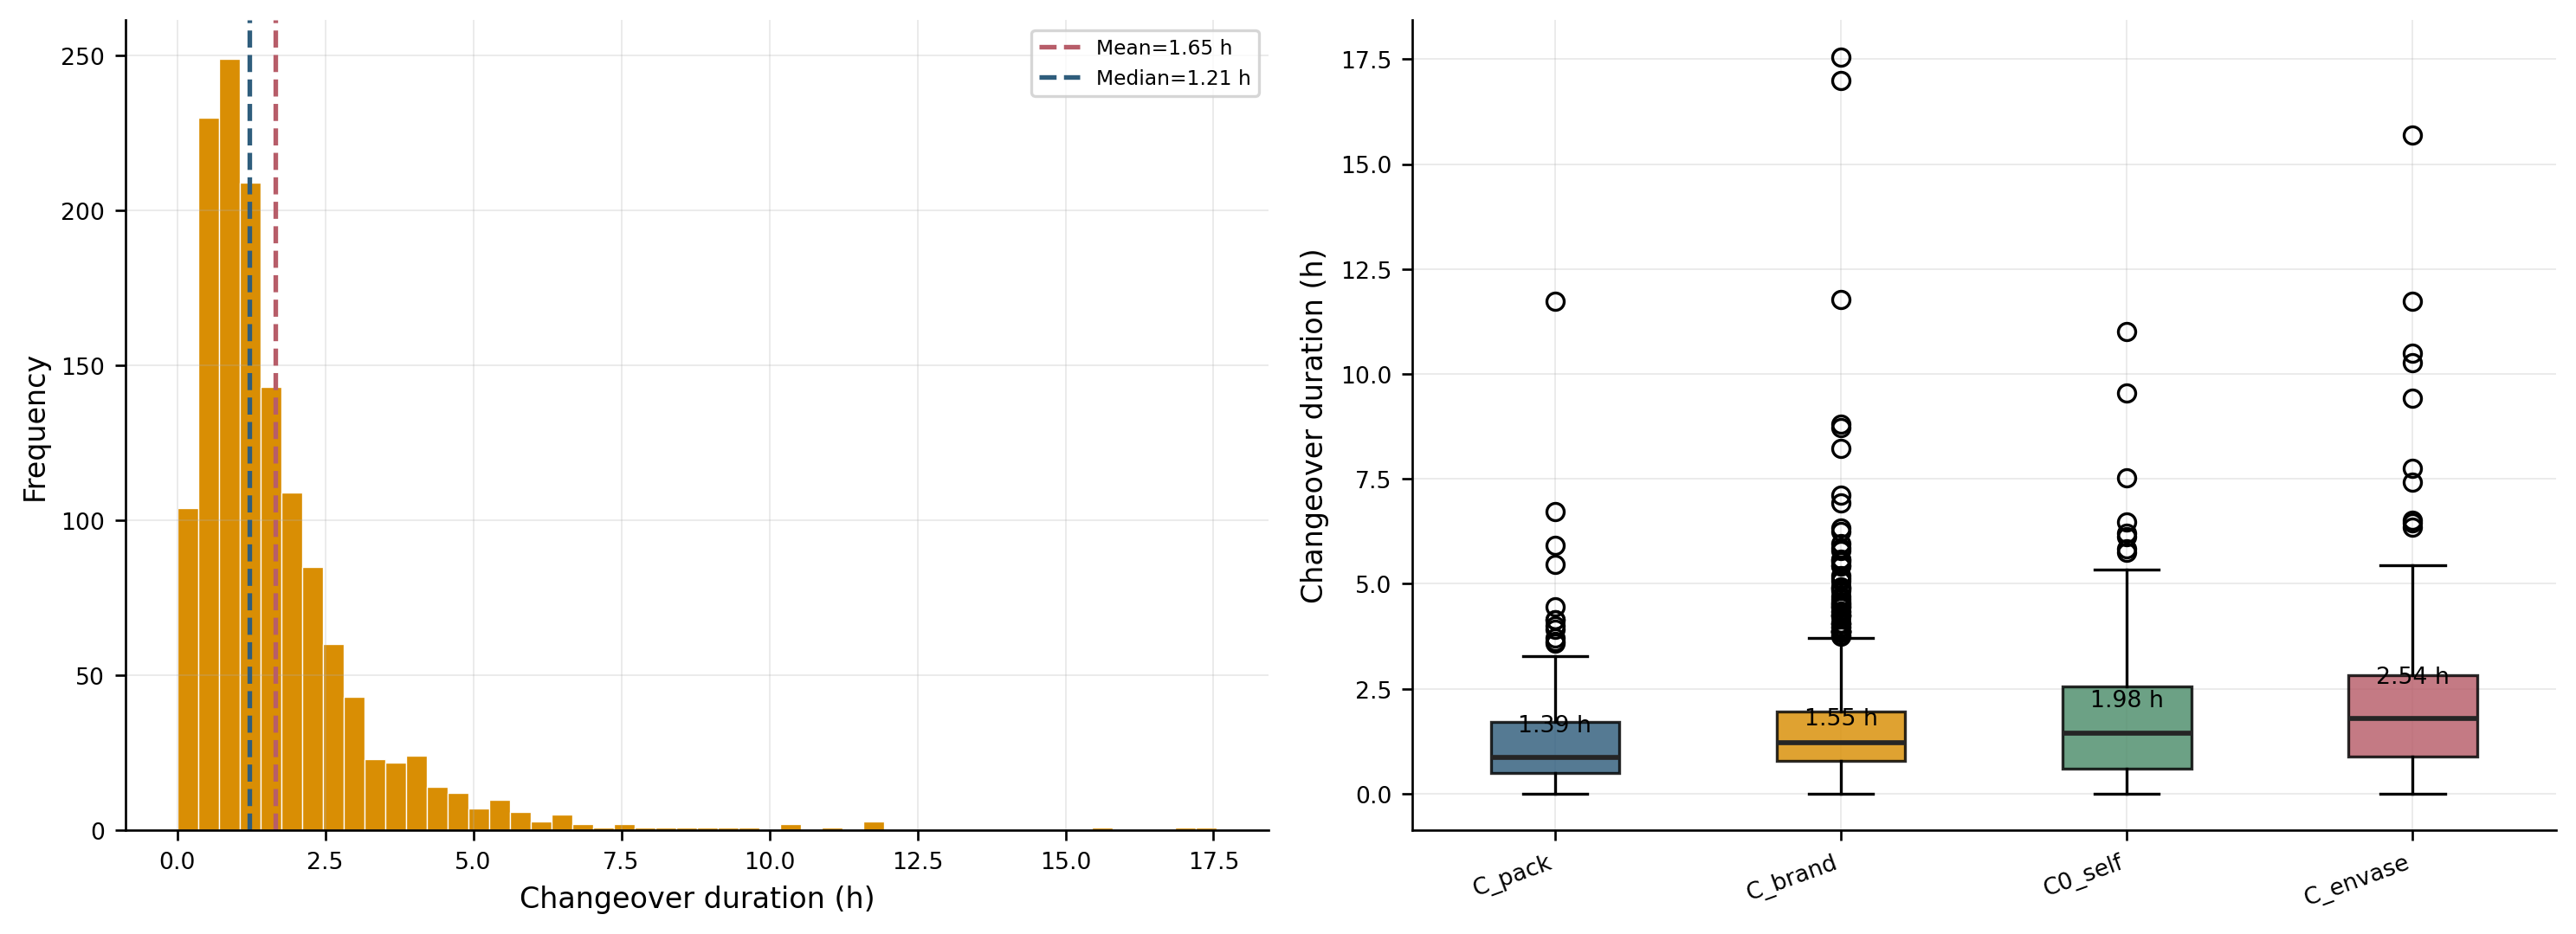
\includegraphics[width=0.9\textwidth]{figures/nb07_fig01.png}
\caption{Global distribution of the $1{,}378$ changeover durations (left) and by
edge type (right). The right skew and the heavier mean of C\_envase versus
C\_pack are already visible and preview the ordering established in
Section~\ref{sec:res-perm}.}
\label{fig:eda}
\end{figure}

% =====================================================================
\section{Problem statement, objectives and hypotheses}\label{sec:problem}
% =====================================================================
\paragraph{The operational problem.}
Let $\mathcal{S}$ be the set of SKUs to produce in a week, each with a fixed
demand $V_i$ (hectolitres), and let $\mathcal{L}=\{14,17,19\}$ be the lines. For
SKU $i$ on line $\ell$ the production time is $V_i/\rho_{i\ell}$, where
$\rho_{i\ell}$ is the throughput (HL/h); putting $j$ immediately after $i$ on
line $\ell$ costs a changeover time $c_{\ell ij}$. Writing $y_{\ell i}=1$ if line
$\ell$ produces $i$ and $x_{\ell ij}=1$ if $i$ immediately precedes $j$ on
$\ell$, the weekly hours of line $\ell$ are
\begin{equation}
H_\ell \;=\; s_\ell + \sum_{i} y_{\ell i}\,\frac{V_i}{\rho_{i\ell}}
            \;+\; \sum_{i\neq j} x_{\ell ij}\,c_{\ell ij},
\label{eq:hours}
\end{equation}
with start-up $s_\ell$. The planner must keep $H_\ell\le \kappa_\ell$ (capacity
$\kappa_{14}=110$, $\kappa_{17}=\kappa_{19}=115$\,h), respect format eligibility,
and honour urgent orders. \emph{Minimising $\sum_\ell H_\ell$ is equivalent to
maximising the slack $\sum_\ell(\kappa_\ell-H_\ell)$ and, because the only
movable term is the changeover sum, to minimising changeover loss --- hence to
protecting OEE.} The whole pipeline therefore hinges on a credible estimate of
$c_{\ell ij}$, which is exactly what the statistical analysis provides.

\paragraph{Objectives.}
\begin{description}[leftmargin=2.2em,itemsep=1pt]
\item[O1] Identify, per changeover type, the parametric law that best describes
its duration (model identification).
\item[O2] Build a defensible, \emph{self-updating} cost per changeover usable as a
Bayesian prior for next-year planning, and verify it remains valid out of sample.
\item[O3] Test whether changeover types and lines can be \emph{ordered} by
difficulty, so the optimiser can be steered with a few interpretable rules.
\item[O4] Quantify the operational impact (lost hL, recovered slack, urgency
feasibility) of acting on these results through the scheduler.
\end{description}

\paragraph{Statistical hypotheses.}
The two methods translate into four formally testable hypotheses.
\begin{description}[leftmargin=3.2em,itemsep=2pt]
\item[\textbf{H1}] \emph{(model identification)} Each edge-type duration follows an
identifiable positive-skew family among Gamma, Weibull, LogNormal and Inverse
Gaussian. Selection is by AIC; KS and CvM provide diagnostics.
\item[\textbf{H2}] \emph{(stationarity)} The duration distribution is stable
between $H_1$ (Jan--Jun) and $H_2$ (Jul--Dec):
$H_0\!: F_{H_1}=F_{H_2}$ vs. $H_A\!: F_{H_1}\neq F_{H_2}$, tested with two-sample
KS, AD and CvM. Non-rejection licenses using $H_1$ as an informative prior.
\item[\textbf{H3}] \emph{(ordered edge types)} $H_0\!:$ the four types share one
distribution; $H_A\!: m_{\text{C\_pack}}\le m_{\text{C\_brand}}\le m_{\text{C0\_self}}
\le m_{\text{C\_envase}}$, with at least one strict inequality.
\item[\textbf{H4}] \emph{(ordered lines)} $H_0\!: m_{\text{L17}}=m_{\text{L19}}=
m_{\text{L14}}$ vs. $H_A\!: m_{\text{L17}}\le m_{\text{L19}}\le m_{\text{L14}}$.
\end{description}

\paragraph{Eligibility and urgencies.}
Two side constraints shape the feasible region. \emph{Format eligibility} is
physical: line~14 runs $\{1/2,1/3\}$, line~17 only $1/3$, line~19
$\{1/2,1/3,2/5\}$, and --- a stricter, data-driven rule we adopt --- a SKU is
admissible on a line only if that exact SKU was produced there in 2025, so the
optimiser never invents an untested pairing. \emph{Urgencies} are mandatory orders
that must appear early in a line's sequence; we encode them as a hard upper bound
on the position variable ($u_{\ell i}\le 2$). When an urgency cannot be honoured
without violating format, eligibility or capacity, the tool returns
\emph{infeasible} rather than a fabricated schedule --- the only acceptable
behaviour for a planning aid that operators must trust.

\paragraph{Information available.}
Beyond the 2025 history we have the target week (18--22 May 2026): $28$ SKUs and
$36{,}933$\,hL of demand, plus the as-built production log of that week, used in
Section~\ref{sec:res-applied} for a plan-versus-reality reconciliation.

% =====================================================================
\section{Statistical methodology}\label{sec:methods}
% =====================================================================
We use two complementary families of techniques. Method~1 is parametric and
Bayesian; Method~2 is non-parametric and permutation-based. Both are deliberately
distribution-aware: the strong right skew of the response (Fig.~\ref{fig:eda})
makes normal-theory tools (ANOVA, $t$-tests) inappropriate.

\paragraph{Why these two, and why together.}
The choice is dictated by the two questions the business asks. ``\emph{How long
will this changeover take, and how sure are we?}'' is an estimation question with
a need for uncertainty attached to the edge cost of the Bayesian complex network.
``\emph{Is type/line $A$ really worse than $B$?}'' is a testing question where we
refuse to assume a Gaussian shape. Method~1 supplies the probabilistic edge costs
that the optimiser consumes; Method~2 certifies the qualitative ordering that
makes those costs interpretable.

\subsection{Method 1 --- Goodness-of-fit and Bayesian MCMC updating}\label{sec:m1}

\subsubsection{Temporal split}
The statistical duration dataset is split chronologically:
\[
H_1=\text{January--June 2025}, \qquad
H_2=\text{July--December 2025}.
\]
The first half, $H_1$, is used to choose the duration family and initialise the
informative Bayesian model. The second half, $H_2$, is used to validate the model
and to update the posterior. This mirrors the planning situation: the plant has
historical evidence and wants to know how it should inform future weeks.

\subsubsection{Candidate duration families}
Changeover durations are positive and right-skewed, so we consider four positive
families:
\begin{align*}
\text{Gamma}(\alpha,\theta):&\ f(x)=\tfrac{1}{\Gamma(\alpha)\theta^\alpha}x^{\alpha-1}e^{-x/\theta},
&\text{Weibull}(k,\lambda):&\ f(x)=\tfrac{k}{\lambda}\big(\tfrac{x}{\lambda}\big)^{k-1}e^{-(x/\lambda)^k},\\
\text{LogNormal}(\mu,\sigma):&\ f(x)=\tfrac{1}{x\sigma\sqrt{2\pi}}e^{-\frac{(\ln x-\mu)^2}{2\sigma^2}},
&\text{InvGauss}(\mu,\lambda):&\ f(x)=\sqrt{\tfrac{\lambda}{2\pi x^3}}\,e^{-\frac{\lambda(x-\mu)^2}{2\mu^2 x}} .
\end{align*}
All families are fitted by maximum likelihood using \texttt{scipy.stats}. Since
SciPy adds an extra location parameter \texttt{loc} to continuous distributions,
we fix it at zero (\texttt{floc=0}). This forces the fitted distributions to
start at zero hours, which is appropriate because changeover durations cannot be
negative.

\subsubsection{Selection rule: GoF filter followed by AIC}
For each edge type $g$ and candidate family $f$, we fit the parameters
$\hat\theta_{gf}$ on $H_1$ and compute Akaike's Information Criterion
\cite{akaike1974},
\begin{equation}
\text{AIC}_{gf}=-2\,\ell(\hat\theta_{gf})+2k,
\label{eq:aic}
\end{equation}
with $k=2$ free parameters. We also compute the one-sample Kolmogorov--Smirnov
\cite{massey1951} and Cram\'er--von Mises \cite{anderson1962cvm} diagnostics,
\begin{equation}
D=\sup_x\big|F_n(x)-F_{\hat\theta}(x)\big|,\qquad
W^2=\!\int\!\big[F_n(x)-F_{\hat\theta}(x)\big]^2\,dF_{\hat\theta}(x).
\label{eq:ks}
\end{equation}
The selection rule is deliberately conservative:
\[
\mathcal A_g=\{f:\ p^{KS}_{gf}>0.05\ \text{and}\ p^{CvM}_{gf}>0.05\},
\qquad
f_g^\star=\arg\min_{f\in\mathcal A_g}\text{AIC}_{gf}.
\]
If $\mathcal A_g$ is empty, we use the lowest-AIC family as a diagnostic fallback
and report that no family passed the GoF filter. This happens only for the
data-rich C\_brand group, where the tests are over-powered enough to reject even
small deviations.

\subsubsection{Bayesian posterior on the selected family}
The selected family is not merely descriptive: it is the duration model used for
Bayesian updating. For edge type $g$,
\[
X_i\mid\theta_g \sim f_g^\star(x_i\mid\theta_g),
\]
where $\theta_g$ contains the two positive parameters of the selected family. We
sample on the log-parameter scale,
\[
z_g=\log\theta_g,
\]
with a weak proper prior
\[
z_g\sim\mathcal N(0,5^2 I).
\]
The informative posterior is equivalent to first learning from $H_1$ and then
updating with $H_2$:
\begin{equation}
\pi_I(z_g\mid H_1,H_2)
\propto
\pi_0(z_g)
\prod_{x_i\in H_1} f_g^\star(x_i\mid z_g)
\prod_{x_i\in H_2} f_g^\star(x_i\mid z_g).
\label{eq:posterior_mcmc_inf}
\end{equation}
For comparison, the weak/no-history posterior uses the same weak prior but learns
only from $H_2$:
\begin{equation}
\pi_W(z_g\mid H_2)
\propto
\pi_0(z_g)
\prod_{x_i\in H_2} f_g^\star(x_i\mid z_g).
\label{eq:posterior_mcmc_weak}
\end{equation}
Because Weibull, LogNormal and Inverse Gaussian do not provide the simple closed
form available to conjugate Gamma--Exponential models, both posteriors are
estimated with a Metropolis--Hastings MCMC sampler on $z_g$. Fixed random seeds
make the posterior summaries reproducible.

\paragraph{Cost summary.}
For every MCMC draw we transform the parameters into the expected duration
$m(\theta_g)=\mathbb E[X\mid\theta_g]$:
\[
\begin{array}{ll}
\text{Gamma:} & m=\alpha\theta,\\
\text{Weibull:} & m=\lambda\,\Gamma(1+1/k),\\
\text{LogNormal:} & m=\exp(\mu+\sigma^2/2),\\
\text{InvGauss:} & m=\mu.
\end{array}
\]
The operational cost reported to the optimiser is the posterior median of
$m(\theta_g)$, with the $2.5\%$ and $97.5\%$ quantiles used as a credible
interval. The median is preferred to the posterior mean because LogNormal and
Inverse Gaussian posteriors can be very long-tailed when a group is sparse.

\subsubsection{Stationarity tests}
Whether the $H_1$ information is still useful in $H_2$ is a two-sample
distribution-equality question. We test
\[
H_0:F_{H_1}=F_{H_2},\qquad H_A:F_{H_1}\neq F_{H_2}
\]
with KS, Anderson--Darling \cite{anderson1952} and Cram\'er--von Mises. These
statistics weight the empirical CDF gap differently (Table~\ref{tab:edftests}),
so using all three gives protection against a test that is blind to the departure
present in the data.

\begin{table}[H]\centering\small
\begin{tabular}{@{}p{3.2cm}p{4.2cm}p{5.3cm}@{}}
\toprule
Test & Main sensitivity & Role in the analysis \\
\midrule
Kolmogorov--Smirnov & largest CDF gap & one-sample GoF and $H_1$--$H_2$ stationarity \\
Cram\'er--von Mises & integrated squared CDF gap & one-sample GoF and $H_1$--$H_2$ stationarity \\
Anderson--Darling & tail-weighted CDF gap & stationarity of long-changeover tails \\
\bottomrule
\end{tabular}
\caption{Empirical-distribution-function diagnostics used for model selection
and stationarity.}
\label{tab:edftests}
\end{table}

\subsubsection{Empirical-Bayes per-edge priors}
Individual directed edges are sparse: many product-to-product transitions occur
only once. The type-level MCMC posterior therefore supplies the main cost
distribution, while edge-level information is used where available. Edges with
$n\ge2$ observations in $H_1$ receive an edge-specific Gamma fit as a local
Empirical-Bayes adjustment; edges with fewer observations fall back to the
type/global cost. This is a partial-pooling strategy \cite{gelman2013bda}: trust
the edge where the cell is rich, borrow strength from the population where it is
thin.

\subsection{Method 2 --- Permutation tests for ordered alternatives}\label{sec:m2}
Because the response is heavily skewed and several groups are small, H3--H4 are
tested with \emph{rank-based permutation} procedures that assume nothing about the
shape of the distribution. The logic is exchangeability: \emph{if} $H_0$ holds,
the group labels carry no information, so reshuffling them leaves the joint
distribution unchanged; repeating a statistic over $B=10{,}000$ random relabelings
builds its exact (Monte-Carlo) null distribution \cite{good2005permutation}. The
$p$-value is $(\#\{T^{(b)}\ge T_{\text{obs}}\}+1)/(B+1)$.

\paragraph{Omnibus equality.}
With pooled ranks, mean within-group rank $R_i$, sizes $n_i$ and grand mean
$\bar R$, the dispersion statistic
\begin{equation}
Q=\sum_{i=1}^{k} n_i\,(R_i-\bar R)^2
\end{equation}
detects \emph{any} difference among the $k$ groups (it is the
Kruskal--Wallis numerator, here calibrated by permutation rather than $\chi^2$).

\paragraph{Ordered alternatives.}
A significant $Q$ only says ``some difference''. To test a \emph{direction} we use
order-aware statistics. For the $k=4$ edge types we use the linear rank contrast
\begin{equation}
T=3R_4+R_3-R_2-3R_1,
\end{equation}
whose coefficients $(-3,-1,+1,+3)$ make large $T$ evidence for the increasing
order $m_1\le m_2\le m_3\le m_4$. For the $k=3$ lines we use the
Jonckheere--Terpstra statistic \cite{jonckheere1954,terpstra1952},
\begin{equation}
JT=\sum_{i<j}U_{ij},\qquad
U_{ij}=\#\{(a,b): x_{ia}<x_{jb}\},
\end{equation}
the canonical distribution-free test against an ordered trend, where $U_{ij}$ is
the Mann--Whitney count of how often group $j$ exceeds group $i$.

\paragraph{Post-hoc.}
After a global rejection we localise the effect. For edge types we test each
ordered pair with $T_{ij}=R_j-R_i$ over the $\binom{4}{2}=6$ pairs and control the
family-wise error with Bonferroni ($\alpha=0.05/6=0.0083$). For lines we use
one-sided Mann--Whitney tests \cite{mannwhitney1947} with $\alpha=0.05/3=0.0167$.

% =====================================================================
\section{Results of the statistical analysis}\label{sec:results}
% =====================================================================
The temporal split gives $n_{H_1}=728$ and $n_{H_2}=650$ changeovers.

\subsection{Exploratory analysis}\label{sec:eda}
Before any inference, the shape of the data justifies the modelling choices. The
$1{,}378$ durations are positive, right-skewed and heavy-tailed: the median sits
below the mean for every group (Tables~\ref{tab:typestats} and \ref{tab:lines}),
the classic signature of a process with a floor (a changeover cannot take zero
time) and a long upper tail (occasional very hard changeovers). Skewness is most
pronounced for C\_envase, whose mean ($2.54$\,h) exceeds its median ($1.78$\,h) by
$43\%$, and mildest for C\_pack ($1.39$ vs $0.87$\,h). The five edge types are
also wildly unbalanced --- C\_brand alone is $71\%$ of the data and C\_vol barely
$1.5\%$ --- which is itself informative (brand changes are the everyday event;
volume changes are rare and operationally segregated) and which is precisely why a
rank-based, permutation calibration is preferable to a parametric one that would
be dominated by the largest group. These features --- positivity, skew, imbalance
--- are exactly what Method~1's positive families and Method~2's distribution-free
tests are designed to handle.

\subsection{Method 1 --- family selection, priors and stationarity}
Table~\ref{tab:gof} reports the family selected on $H_1$ using the GoF-filtered
AIC rule of Section~\ref{sec:m1}: among families with KS and CvM $p>0.05$, choose
the lowest AIC. \emph{Gamma is not imposed}: it wins for C\_pack, while Inverse
Gaussian, Weibull and LogNormal win for C\_vol, C0\_self and C\_envase
respectively. C\_brand is the only exception to the GoF filter: with
$n_{H_1}=508$, all four families are rejected by KS/CvM, so the lowest-AIC Gamma
fit is retained as a diagnostic fallback. Figure~\ref{fig:familyselect}
visualises this selection rule.

\paragraph{Reading the fitted shapes.}
The winning families are physically interpretable through their hazard. C0\_self
(lot restart) is best fit by a Weibull with shape $k\approx1.06$, i.e.\ an almost
constant hazard --- a restart is a memoryless re-warm-up. C\_envase (label change)
is LogNormal, a multiplicative-error law with a fat upper tail, matching the
operational reality that most label swaps are quick but a few cascade into long
re-registrations. C\_pack and C\_brand are Gamma with shape $\alpha\approx1.2$
($>1$, so an increasing hazard that eventually saturates). These shapes are not
mere curve-fitting: they tell the planner \emph{why} C\_envase is dangerous --- not
a higher floor but a heavier tail --- which is exactly the kind of changeover SMED
programmes target.

\begin{table}[H]\centering\small
\begin{tabular}{@{}lrlrrrl@{}}
\toprule
Edge type & $n_{H_1}$ & Selected family & AIC & KS\,$p$ & CvM\,$p$ & Rule\\
\midrule
C\_pack   &  79 & Gamma     &  189.2 & 0.520 & 0.413 & accepted \\
C\_brand  & 508 & Gamma     & 1422.7 & 0.000 & 0.000 & fallback \\
C\_vol    &  15 & InvGauss  &   45.9 & 0.909 & 0.914 & accepted \\
C0\_self  &  71 & Weibull   &  221.5 & 0.723 & 0.890 & accepted \\
C\_envase &  55 & LogNormal &  202.2 & 0.879 & 0.903 & accepted \\
\bottomrule
\end{tabular}
\caption{Family selection on $H_1$. The rule is lowest AIC among families passing
both KS and CvM diagnostics ($p>0.05$); C\_brand is retained by lowest-AIC
fallback because no candidate passes both tests.}
\label{tab:gof}
\end{table}

\begin{figure}[H]\centering
\includegraphics[width=\textwidth]{figures/nb07_fig10_family_selection.png}
\caption{Family selection by edge type. Solid bars pass both KS and CvM
diagnostics; hatched bars fail at least one diagnostic. The black star marks the
selected family.}
\label{fig:familyselect}
\end{figure}

\begin{figure}[H]\centering
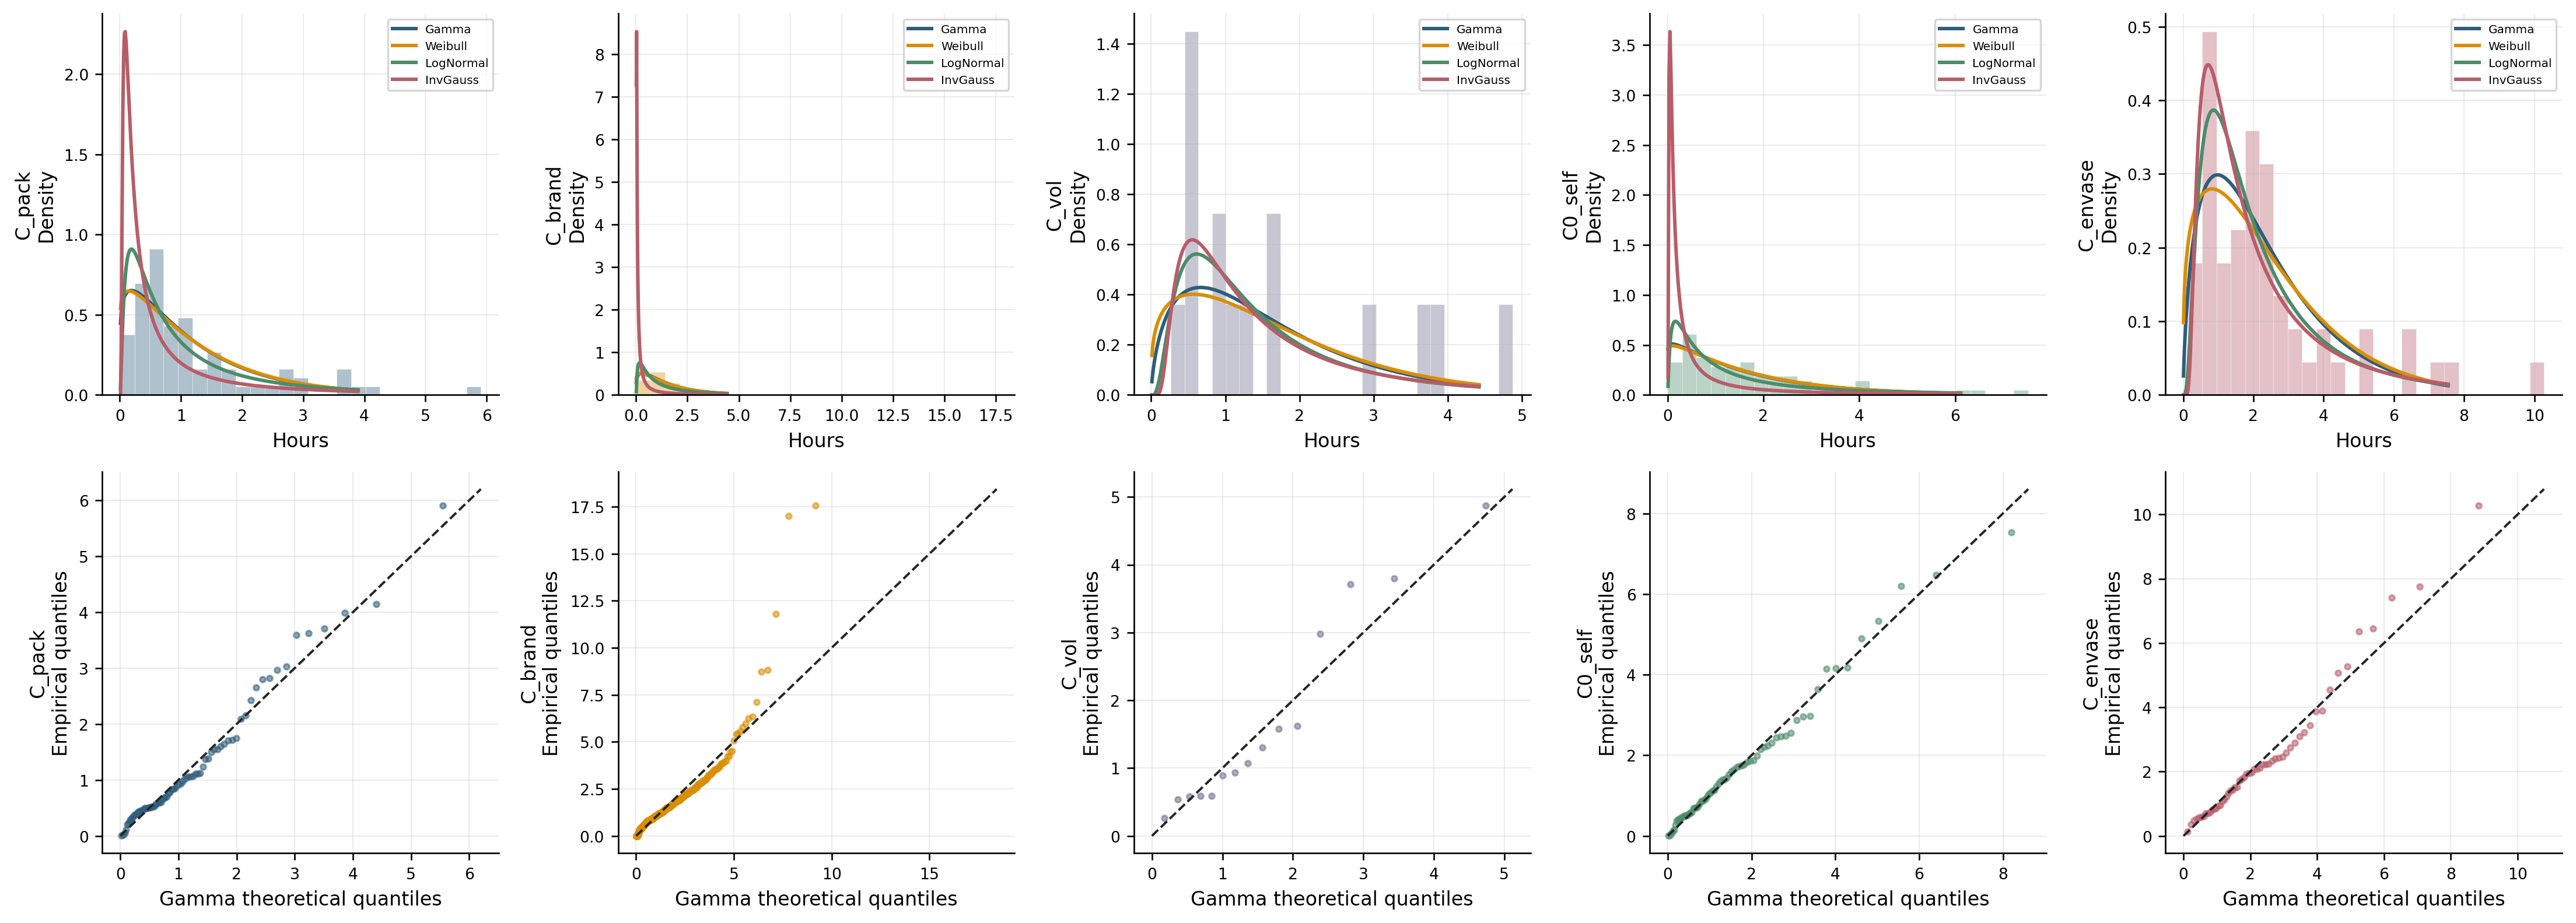
\includegraphics[width=\textwidth]{figures/nb07_fig02.png}
\caption{Per-type histograms on $H_1$ with the four fitted densities (top) and
Gamma QQ-plots (bottom). Points on the diagonal indicate an adequate fit; the
heavier upper tail of C\_envase is apparent.}
\label{fig:goffit}
\end{figure}

\paragraph{Posterior updating.}
The Bayesian update now uses the selected duration family itself. For each edge
type, we sample the posterior of the selected family parameters with
Metropolis--Hastings MCMC and summarise the induced expected duration by its
posterior median (Table~\ref{tab:conv}). The informative posterior combines $H_1$
and $H_2$; the weak posterior learns from $H_2$ only. The comparison is most
stable for data-rich C\_brand (only $-0.05$\,h difference), while sparse or
long-tailed groups show why the historical prior matters: C\_vol has only six
$H_2$ observations and its weak Inverse-Gaussian posterior has a very wide upper
tail; C\_envase inherits the heavy right tail of the selected LogNormal family.
Figures~\ref{fig:mcmccosts}--\ref{fig:mcmcdensity} show the resulting posterior
costs.

\begin{table}[H]\centering\small
\begin{tabular}{@{}llrrrrrr@{}}
\toprule
Edge type & Family & $n_{H_1}$ & $n_{H_2}$ & Informative & Weak & $\Delta$ (h) & 95\% CI (inf.)\\
\midrule
C\_pack   & Gamma     &  79 &  59 & 1.384 & 1.653 & $-0.269$ & [1.184, 1.644]\\
C\_brand  & Gamma     & 508 & 467 & 1.549 & 1.596 & $-0.047$ & [1.469, 1.639]\\
C\_vol    & InvGauss  &  15 &   6 & 1.793 & 2.168 & $-0.375$ & [1.234, 3.668]\\
C0\_self  & Weibull   &  71 &  70 & 1.999 & 2.310 & $-0.311$ & [1.687, 2.403]\\
C\_envase & LogNormal &  55 &  48 & 3.554 & 5.320 & $-1.766$ & [2.599, 5.202]\\
\bottomrule
\end{tabular}
\caption{MCMC posterior expected duration by selected family. Values are
posterior medians in hours; the informative posterior uses $H_1+H_2$, while the
weak posterior uses $H_2$ only.}
\label{tab:conv}
\end{table}

\begin{figure}[H]\centering
\includegraphics[width=\textwidth]{figures/nb07_fig11_mcmc_costs.png}
\caption{Posterior expected duration by selected family. Blue intervals use the
informative $H_1+H_2$ posterior; black intervals use only $H_2$ with a weak prior.}
\label{fig:mcmccosts}
\end{figure}

\begin{figure}[H]\centering
\includegraphics[width=0.9\textwidth]{figures/nb07_fig12_mcmc_density_examples.png}
\caption{Posterior densities of the expected duration for a data-rich type
(C\_brand) and a long-tailed type (C\_envase). The LogNormal posterior for
C\_envase explicitly carries the risk of long label-reference changes.}
\label{fig:mcmcdensity}
\end{figure}

\paragraph{Stationarity (H2).}
Table~\ref{tab:stat} gives the two-sample tests. For four of the five types
($p>0.05$ on all three statistics) we \emph{cannot reject} equality of the $H_1$
and $H_2$ distributions: the process is stationary and the $H_1$-based prior is
valid out of sample. The exception is C\_brand (and, by aggregation, the global
pool), where the very large sample exposes a small but detectable shift --- a
\emph{precision} effect, not a managerially large change, consistent with the
$-2.9\%$ posterior gap in Table~\ref{tab:conv}. A direct $H_1\!\to\!H_2$
re-validation of each selected family (Fig.~\ref{fig:gofvalid}) confirms the same
picture. The empirical-Bayes layer then assigns a specific Gamma prior to $192$ of
the $1{,}015$ edges ($18.9\%$); the remaining $823$ ($81.1\%$) fall back to the
global $\text{Gamma}(\alpha=1.208,\theta=1.295)$, $\mu=1.56$\,h
(Fig.~\ref{fig:ebayes}).

\begin{table}[H]\centering\small
\begin{tabular}{@{}lrrrrrr@{}}
\toprule
Edge type & $n_{H_1}$ & $n_{H_2}$ & KS\,$D$ & KS\,$p$ & AD stat & CvM\,$p$ \\
\midrule
C\_pack   &  79 & 59 & 0.158 & 0.325 & $0.095$  & 0.301 \\
C\_brand  & 508 & 467& 0.089 & 0.039 & $5.170$  & 0.006 \\
C\_vol    &  15 &  6 & 0.233 & 0.938 & $-1.148$ & 0.954 \\
C0\_self  &  71 & 70 & 0.174 & 0.211 & $0.644$  & 0.158 \\
C\_envase &  55 & 48 & 0.154 & 0.516 & $-0.086$ & 0.535 \\
\midrule
GLOBAL    & 728 & 650& 0.093 & 0.005 & $5.856$  & 0.002 \\
\bottomrule
\end{tabular}
\caption{Stationarity ($H_1$ vs $H_2$): two-sample KS, Anderson--Darling and
Cram\'er--von Mises. $p>0.05$ (non-rejection) for every type except the
high-volume C\_brand.}
\label{tab:stat}
\end{table}

\begin{figure}[H]\centering
\begin{subfigure}{0.49\textwidth}\centering
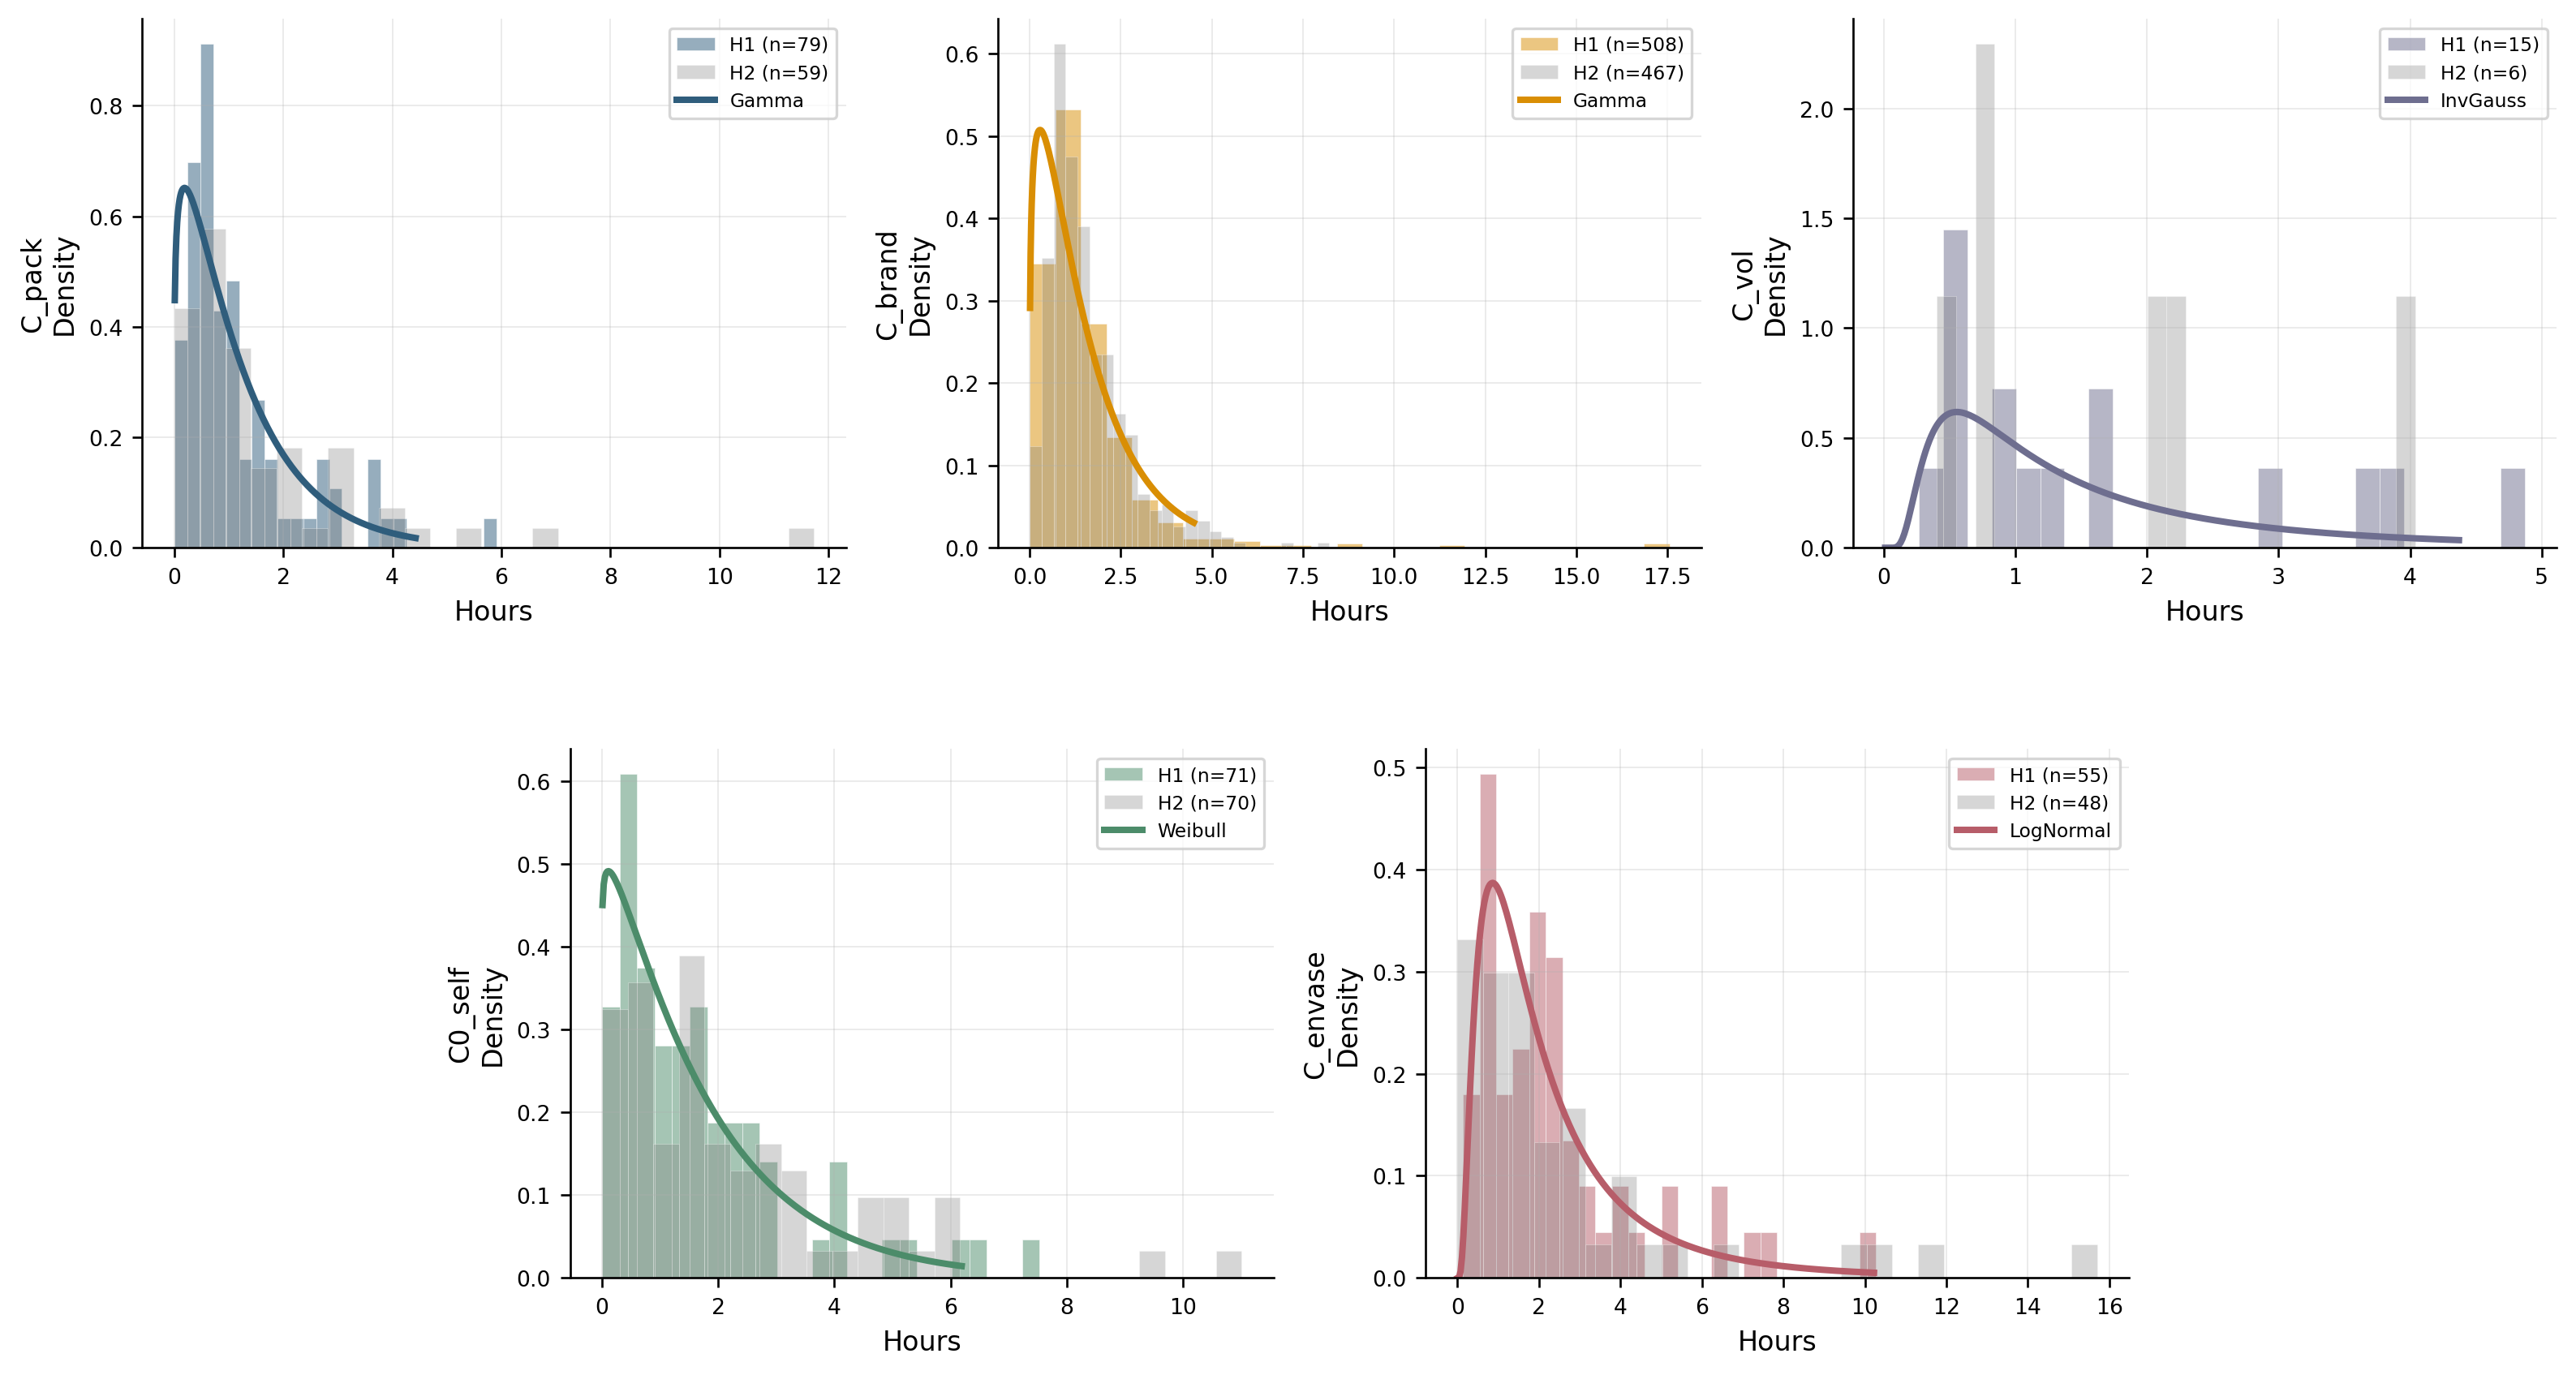
\includegraphics[width=\textwidth]{figures/nb07_fig05.png}
\caption{$H_1\!\to\!H_2$ validation of the selected families.}
\label{fig:gofvalid}
\end{subfigure}\hfill
\begin{subfigure}{0.49\textwidth}\centering
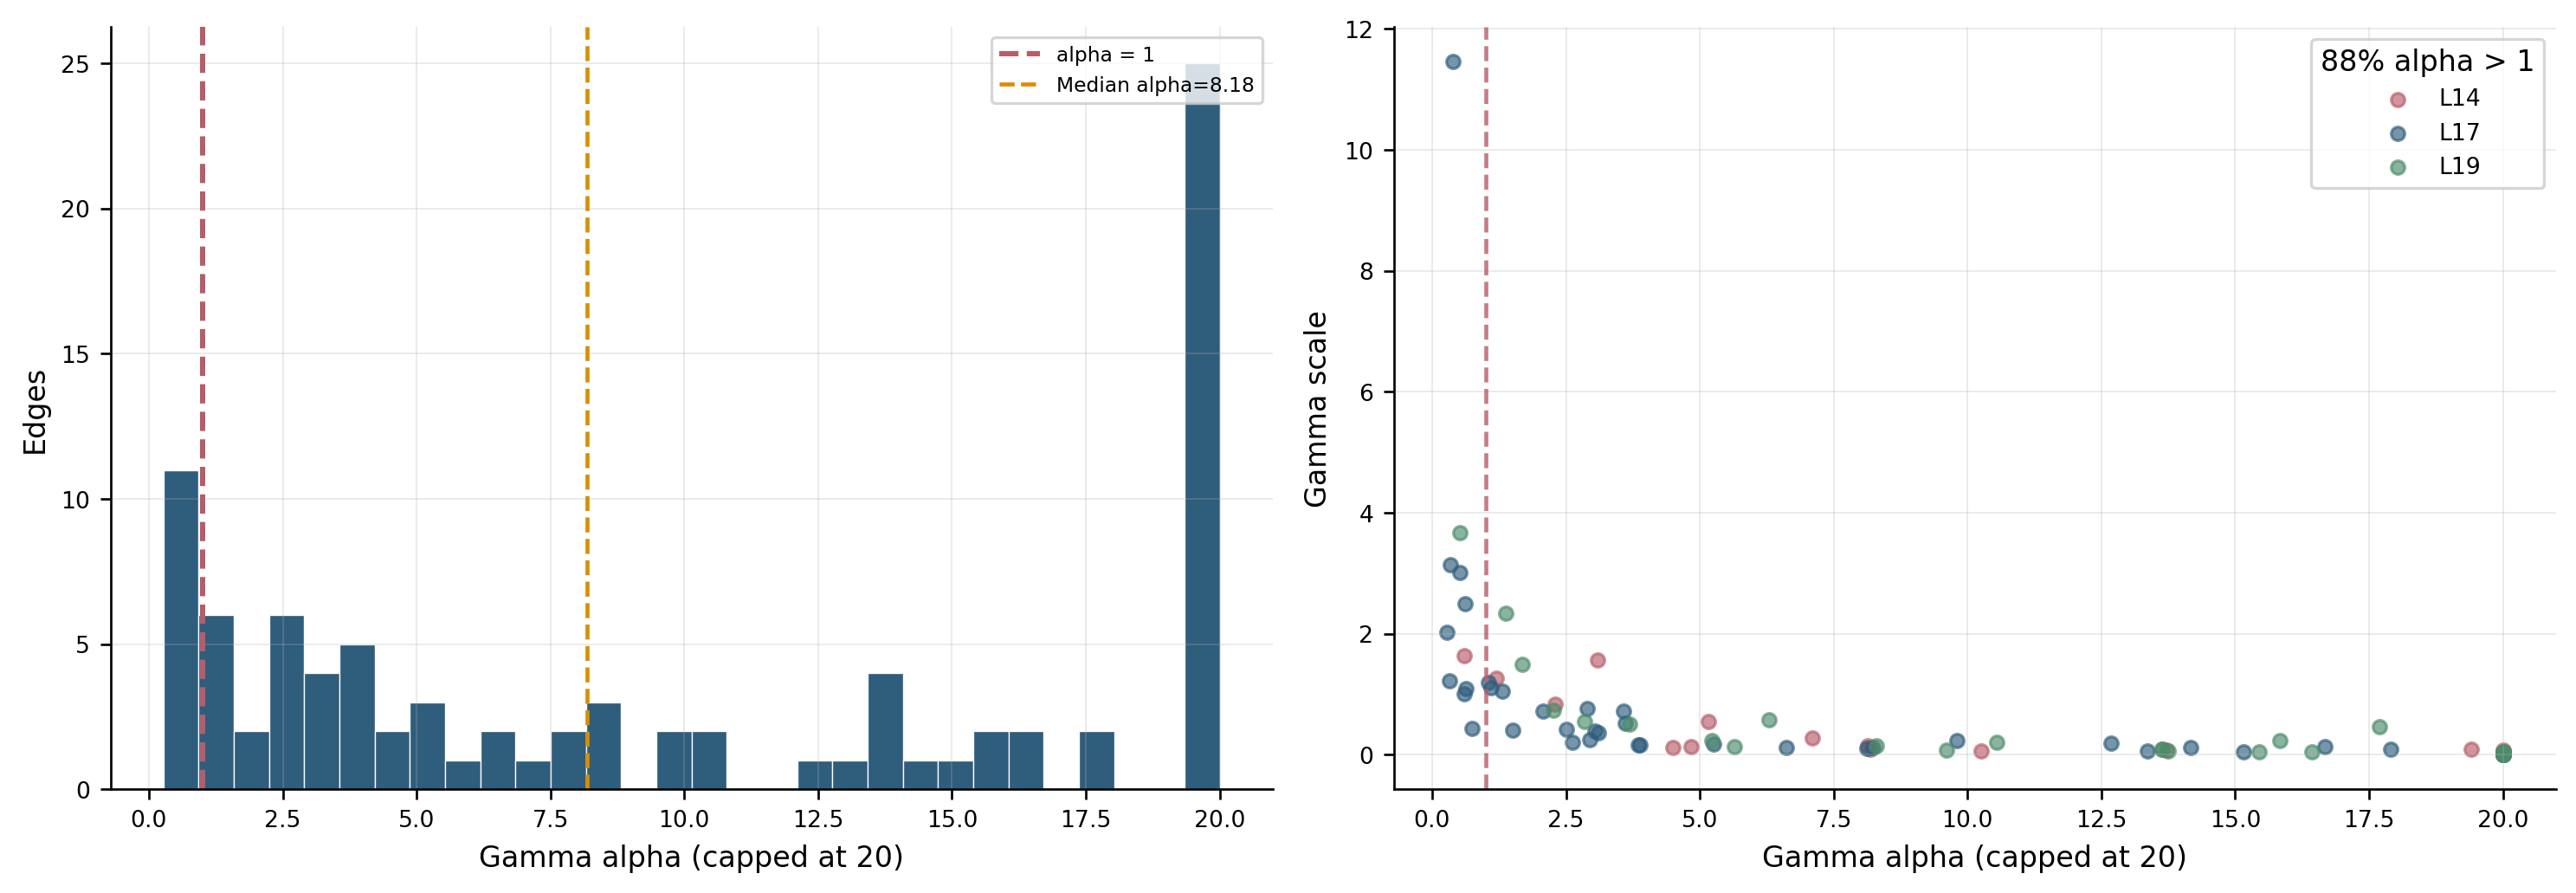
\includegraphics[width=\textwidth]{figures/nb07_fig06.png}
\caption{Per-edge empirical-Bayes Gamma priors.}
\label{fig:ebayes}
\end{subfigure}
\caption{Out-of-sample fit and hierarchical priors. Left: the family chosen on
$H_1$ still describes $H_2$ for the stationary types. Right: distribution of the
per-edge shape parameters; most edges fall back to the global prior.}
\end{figure}

\subsection{Method 2 --- ordered differences between types and lines}\label{sec:res-perm}
\paragraph{Edge types (H3).}
On the full sample the four edge types have clearly increasing mean ranks
(Table~\ref{tab:typestats}). The omnibus permutation test overwhelmingly rejects
equality ($Q=4.67\times10^{6}$, $p=10^{-4}$), and the ordered contrast confirms
the hypothesised direction ($T=863.1$, $p=10^{-4}$; Fig.~\ref{fig:perm-type}). The
Bonferroni post-hoc (Table~\ref{tab:posthoc}) shows the ordering is driven by the
\emph{extremes}: every contrast involving C\_pack (cheapest) or C\_envase (most
expensive) is significant, whereas the adjacent middle pairs
C\_brand\,$\le$\,C0\_self and C0\_self\,$\le$\,C\_envase are not --- brand changes
and lot restarts sit on a statistical plateau. The headline result is that
\textbf{C\_envase ($\mu=2.54$\,h) is significantly more expensive than C\_brand
($\mu=1.55$\,h)}: swapping a label reference costs more than switching brand
entirely, an unintuitive finding with direct sequencing consequences.

\begin{table}[H]\centering\small
\begin{minipage}[t]{0.44\textwidth}\centering
\begin{tabular}{@{}lrrrr@{}}
\toprule
Edge & $n$ & Mean & Median & $R_i$ \\
\midrule
C\_pack   & 138 & 1.389 & 0.870 & 555.1 \\
C\_brand  & 975 & 1.550 & 1.208 & 674.1 \\
C0\_self  & 141 & 1.981 & 1.435 & 727.8 \\
C\_envase & 103 & 2.537 & 1.784 & 824.9 \\
\bottomrule
\end{tabular}
\caption{Duration statistics and mean ranks by edge type.}
\label{tab:typestats}
\end{minipage}\hfill
\begin{minipage}[t]{0.52\textwidth}\centering
\begin{tabular}{@{}lrrl@{}}
\toprule
Ordered pair & $\Delta$mean & $p_{\text{Bonf}}$ & Sig.\\
\midrule
C\_pack\,$\le$\,C\_brand   & 0.161 & 0.0030 & yes \\
C\_pack\,$\le$\,C0\_self   & 0.592 & 0.0066 & yes \\
C\_pack\,$\le$\,C\_envase  & 1.148 & 0.0006 & yes \\
C\_brand\,$\le$\,C0\_self  & 0.431 & 0.352  & no  \\
C\_brand\,$\le$\,C\_envase & 0.987 & 0.0012 & yes \\
C0\_self\,$\le$\,C\_envase & 0.556 & 0.231  & no  \\
\bottomrule
\end{tabular}
\caption{Ordered post-hoc (permutation, Bonferroni $\alpha=0.0083$).}
\label{tab:posthoc}
\end{minipage}
\end{table}

\begin{figure}[H]\centering
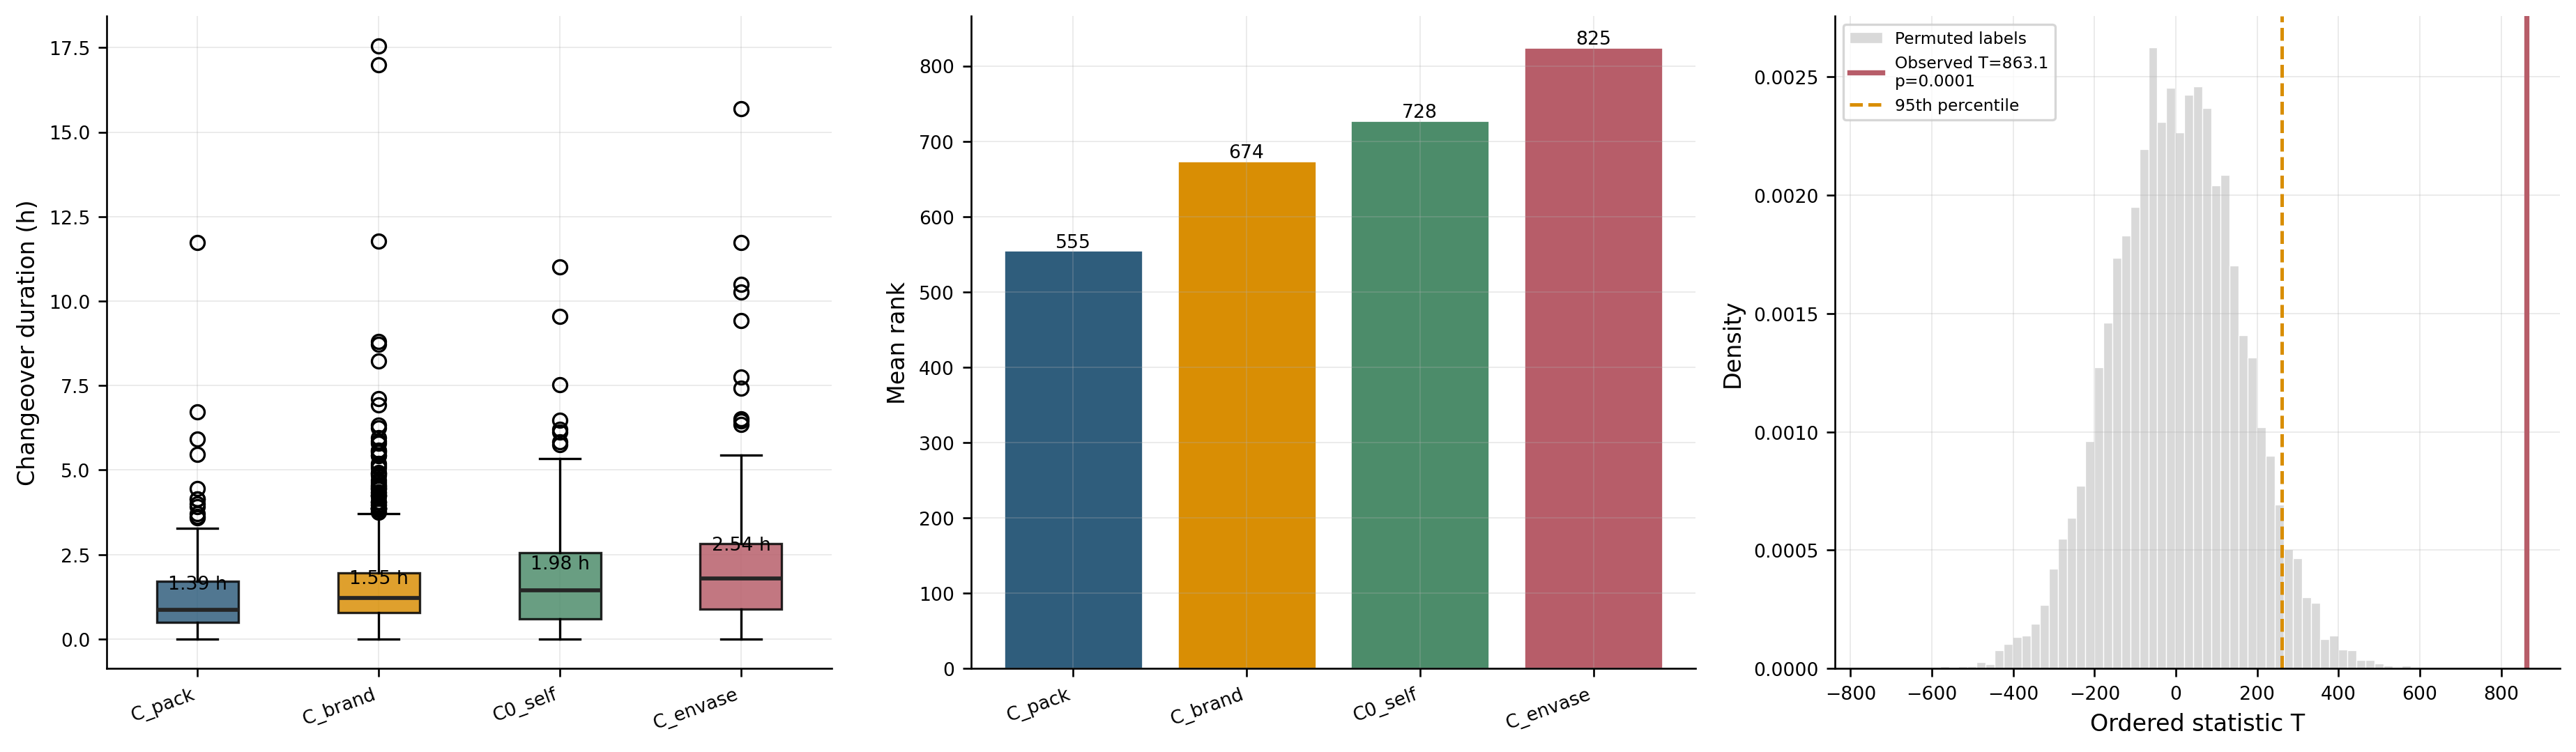
\includegraphics[width=\textwidth]{figures/nb07_fig07.png}
\caption{Application A (edge types). From left: boxplots, mean ranks, omnibus null
distribution of $Q$, and null distribution of the ordered statistic $T$. The
observed statistics lie far in the right tail of their permutation nulls.}
\label{fig:perm-type}
\end{figure}

\begin{figure}[H]\centering
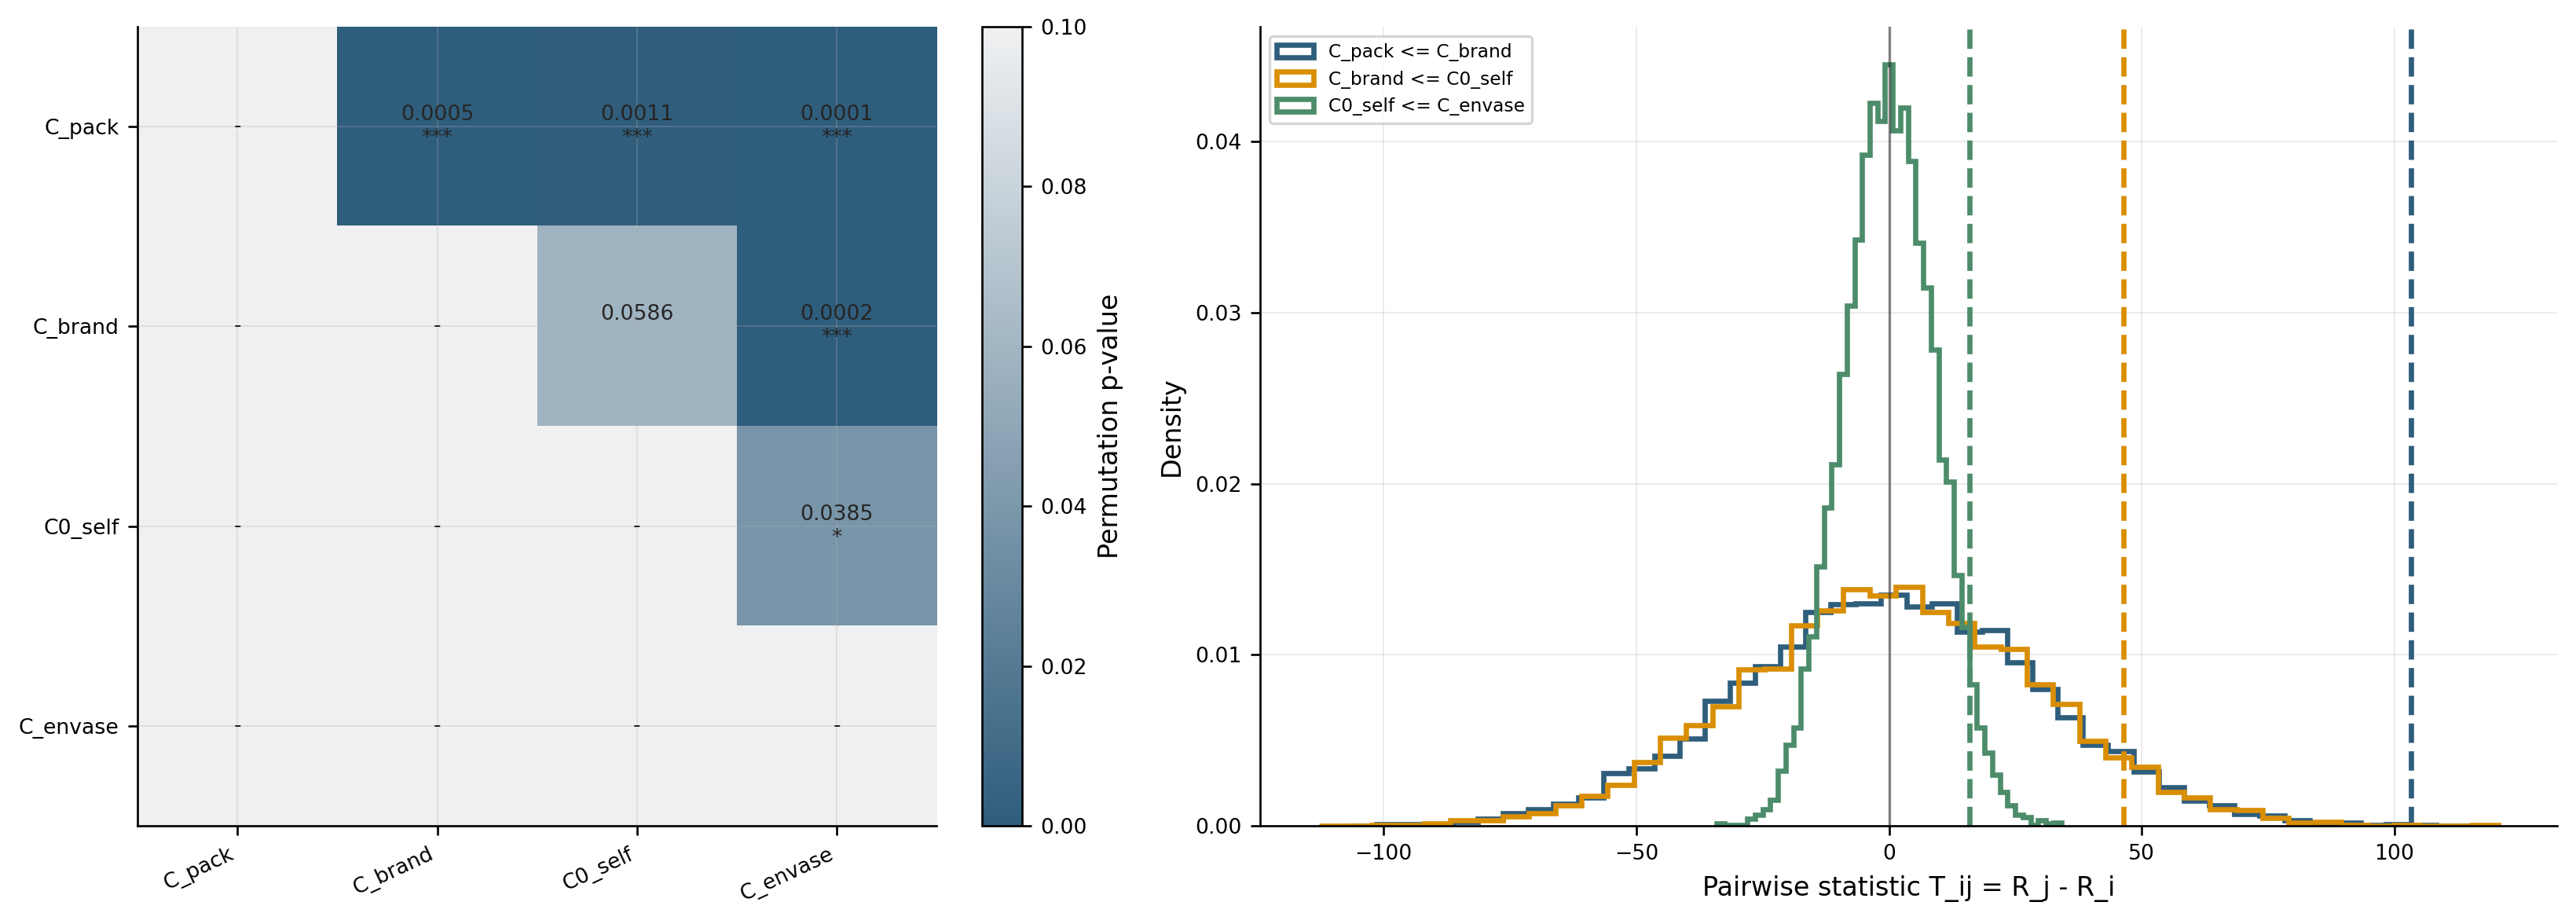
\includegraphics[width=0.95\textwidth]{figures/nb07_fig08.png}
\caption{Ordered post-hoc for edge types. Left: matrix of one-sided permutation
$p$-values for each ordered pair $i\le j$ (green $=$ significant after Bonferroni).
Right: null distributions of the adjacent contrasts that define the proposed
chain. The significant cells trace the path C\_pack $\to$ C\_brand $\to$ C\_envase.}
\label{fig:perm-posthoc}
\end{figure}

\paragraph{Lines (H4).}
The Jonckheere--Terpstra test rejects equality of the three lines
($JT=324{,}709$, $p=3\times10^{-4}$; Fig.~\ref{fig:perm-line}). The post-hoc
(Tables~\ref{tab:lines}--\ref{tab:lines-posthoc}) localises the effect: L14 is
significantly slower than both L17 and L19 ($p<10^{-4}$), while L17 and L19 are
statistically indistinguishable ($p=0.195$). Line~14 is therefore the bottleneck
for long changeovers and should be loaded with sequences that minimise expensive
(label-switching) transitions.

\begin{table}[H]\centering\small
\begin{minipage}[t]{0.44\textwidth}\centering
\begin{tabular}{@{}lrrrr@{}}
\toprule
Line & $n$ & Mean & Median & $R_i$ \\
\midrule
L17 & 609 & 1.580 & 1.150 & 659.1 \\
L19 & 547 & 1.560 & 1.179 & 677.7 \\
L14 & 222 & 2.087 & 1.585 & 801.9 \\
\bottomrule
\end{tabular}
\caption{Duration statistics and mean ranks by line.}
\label{tab:lines}
\end{minipage}\hfill
\begin{minipage}[t]{0.52\textwidth}\centering
\begin{tabular}{@{}lrl@{}}
\toprule
Contrast & $p$ (one-sided) & Sig.\\
\midrule
L17 $<$ L19 & 0.195   & ns   \\
L17 $<$ L14 & $<10^{-5}$ & *** \\
L19 $<$ L14 & $3\times10^{-5}$ & *** \\
\bottomrule
\end{tabular}
\caption{Mann--Whitney post-hoc (Bonferroni $\alpha=0.0167$).}
\label{tab:lines-posthoc}
\end{minipage}
\end{table}

\begin{figure}[H]\centering
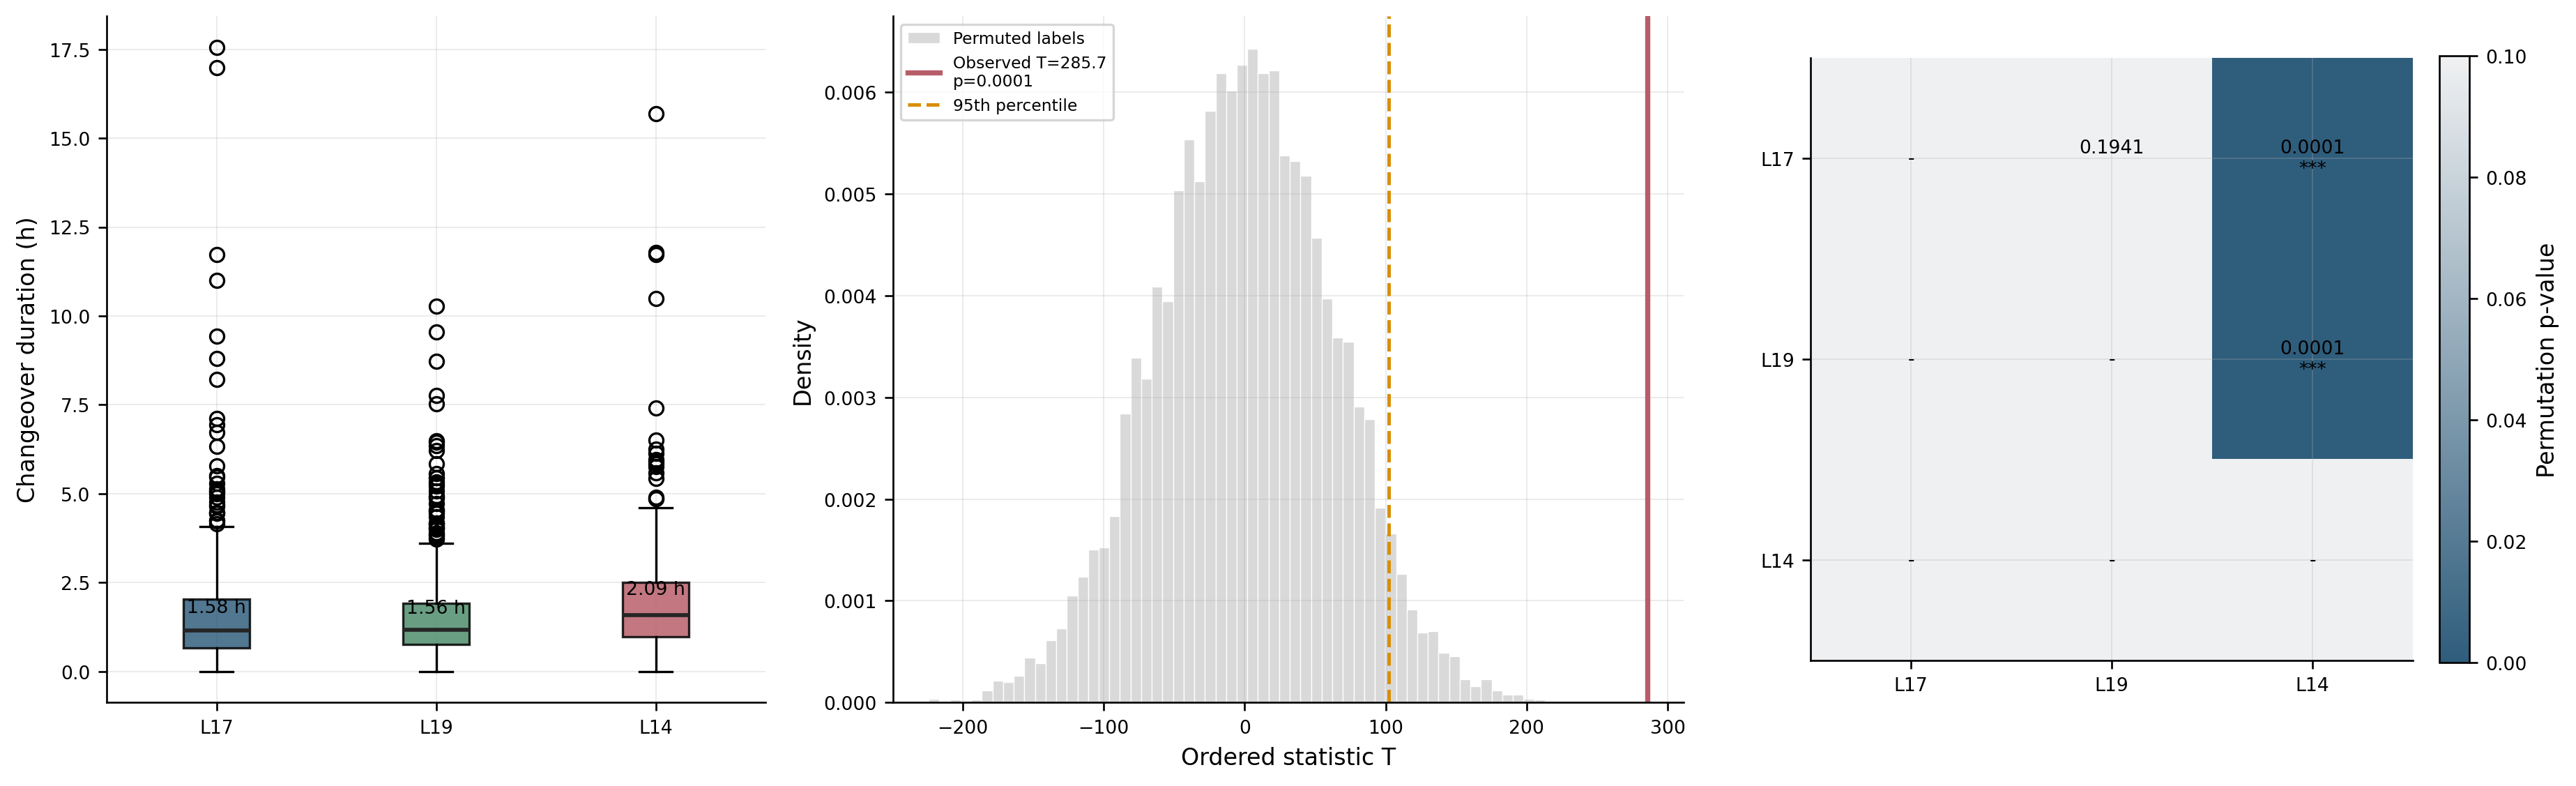
\includegraphics[width=0.82\textwidth]{figures/nb07_fig09.png}
\caption{Application B (lines): boxplots by line and the Jonckheere--Terpstra null
distribution with the observed $JT$ far in the right tail.}
\label{fig:perm-line}
\end{figure}

\paragraph{Synthesis.}
Table~\ref{tab:summary} collects the four decisions. Method~1 delivers a
validated, self-updating cost per changeover; Method~2 certifies how to order
those costs. Both point the same way and feed directly into the optimiser of
Section~\ref{sec:optim}.

\begin{table}[H]\centering\small\setlength{\tabcolsep}{4.5pt}
\begin{tabular}{@{}llll@{}}
\toprule
Method & $H_0$ / $H_A$ & Statistic & Decision \\
\midrule
GoF (global, validated on $H_2$) & selected family vs.\ alt. & $\text{AIC}_{H_2}=2022.4$ & Gamma retained \\
Stationarity (per type)          & $F_{H_1}=F_{H_2}$               & KS/AD/CvM            & not rejected (4/5 types) \\
Omnibus permutation ($k=4$)      & all labels exchangeable          & $Q=4.67\times10^{6}$ & reject $H_0$ ($p=10^{-4}$) \\
Ordered contrast ($k=4$)         & C\_pack$\le\cdots\le$C\_envase    & $T=863.1$            & reject $H_0$ ($p=10^{-4}$) \\
Jonckheere--Terpstra ($k=3$)     & L17$\le$L19$\le$L14              & $JT=324{,}709$       & reject $H_0$ ($p=3\!\times\!10^{-4}$) \\
\bottomrule
\end{tabular}
\caption{Summary of the four hypothesis tests and their decisions.}
\label{tab:summary}
\end{table}

% =====================================================================
\section{Optimization: methodology and results}\label{sec:optim}
% =====================================================================
The statistical model is only useful if it changes a decision. This section turns
the validated changeover cost into a weekly schedule. We first build the cost
itself from a directed-graph post-mortem, then state three interchangeable
optimisation engines, and finally report their results and a confrontation with
reality.

\subsection{From history to cost: the directed-graph post-mortem}\label{sec:postmortem}
For optimisation we need a number on every arc $i\!\to\!j$. We treat each
historical transition as a sample of OEE \emph{degradation},
\begin{equation}
\delta_{ij}=\overline{\text{OEE}}_{\text{expected}}-\text{OEE}_{\text{observed}}(i\!\to\!j),
\end{equation}
and flag an arc as a \textbf{black spot} when it is both recurrent ($\text{count}\ge2$)
and an outlier in degradation,
\begin{equation}
\delta_{ij}>\mu_\delta+1.5\,\sigma_\delta ,
\label{eq:blackspot}
\end{equation}
a robust $1.5\sigma$ rule on the line's degradation distribution. The avoidable
loss of an arc is estimated as
\begin{equation}
\widehat{\text{hL lost}}_{ij}=\delta_{ij}\times \text{hL}_{ij},
\end{equation}
the degradation scaled by the volume that flowed through it. The same transition
matrix is read as a directed graph $G_\ell=(N_\ell,E_\ell)$ per line, on which we
compute weighted in/out-degree, betweenness and PageRank to rank ``hard-to-reach''
destination nodes. Graph densities are low ($0.060$, $0.065$, $0.041$ for
L14/L17/L19), i.e.\ each product only ever follows a handful of others --- a
structure the optimiser exploits to find cheap neighbours. The arc cost that
enters the optimiser is either this OEE degradation (CP-SAT objective) or its
translation into changeover \emph{hours} via Eq.~\eqref{eq:hours} (graph/GA
objective); at fixed volume the two are monotone, since worse OEE means more real
time for the same output.

\subsection{Estimating the model parameters $\rho_{i\ell}$ and $c^h_{\ell ij}$}\label{sec:params}
Equation~\eqref{eq:hours} needs two estimated quantities per line. The
\textbf{throughput} $\rho_{i\ell}$ is the \emph{median} HL/h of SKU $i$ on line
$\ell$ across its 2025 orders,
\begin{equation}
\hat\rho_{i\ell}=\operatorname{median}\{\text{HL/h}:(\text{SKU}=i,\text{line}=\ell)\},
\end{equation}
the median being far more robust than the mean to the occasional bad shift; when a
pair $(i,\ell)$ has no history we back off to the SKU's plant-wide median and then
to the plant mean, with a hard floor of $20$\,HL/h. The estimated medians are
$82.4$, $144.2$ and $140.5$\,HL/h for L14, L17 and L19 --- L14 is intrinsically the
slowest line, compounding the changeover penalty established in
Section~\ref{sec:res-perm}. The \textbf{changeover hours} $c^h_{\ell ij}$ are the
posterior summaries of the selected-family Bayesian model (Section~\ref{sec:m1}), looked up
on the arc $\text{node}(i)\!\to\!\text{node}(j)$; a missing arc falls back to the
line-mean changeover, inflated by a factor $2.5$ when the formats differ, and the
result is clipped to $[0,12]$\,h to bound simulator pathologies.

\subsection{Engine 1 --- exact CP-SAT integer program}
The exact model is a capacitated assignment-plus-sequencing program solved with
Google OR-Tools CP-SAT \cite{perron2023ortools}. With binaries $y_{\ell i}$
(assignment), $x_{\ell ij}$ (immediate succession) and integer position variables
$u_{\ell i}$, and arc cost $c_{\ell ij}$ from Section~\ref{sec:postmortem},
\begin{align}
\min\ &\sum_{\ell,i,j} c_{\ell ij}\,x_{\ell ij} \label{eq:cpobj}\\[-1pt]
\text{s.t.}\ \ &\sum_{\ell} y_{\ell i}=1 &&\forall i &&\text{(each SKU produced once)}\\
&\sum_{j} x_{\ell ij}=y_{\ell i},\ \ \sum_{j} x_{\ell ji}=y_{\ell i} &&\forall \ell,i &&\text{(flow conservation, virtual start/end)}\\
&u_{\ell i}-u_{\ell j}+|\mathcal{S}|\,x_{\ell ij}\le |\mathcal{S}|-1 &&\forall \ell,i\neq j &&\text{(MTZ sub-tour elimination)}\\
&s_\ell+\sum_i y_{\ell i}\tfrac{V_i}{\rho_{i\ell}}+\sum_{i\neq j} c^{h}_{\ell ij}x_{\ell ij}\le \kappa_\ell &&\forall \ell &&\text{(weekly capacity)}\\
&y_{\ell i}=0\ \text{if format}(i)\notin \mathcal{F}_\ell;\quad u_{\ell i}\le 2\ \text{if $i$ urgent} && &&\text{(eligibility, urgencies)}
\end{align}
The Miller--Tucker--Zemlin constraints \cite{miller1960mtz} forbid disconnected
cycles so that each line's selected arcs form a single Hamiltonian path; the
position variables double as the lever to force urgent SKUs early. The solver runs
with a $60$\,s budget and a feasible heuristic warm-start (used only to seed the
search, not to bias the optimum). This engine optimises OEE degradation directly
through Eq.~\eqref{eq:cpobj}.

\subsection{Engine 2 --- behaviour-graph hours model}
The second engine reformulates the objective as \emph{hours} rather than
degradation, which is what the plant ultimately budgets. It learns one directed
behaviour graph per line from 2025, with arc weight equal to the expected
transition hours, and applies a strict eligibility rule: a SKU is admissible on a
line only if (i) its physical format is allowed
($\mathcal F_{14}=\{1/2,1/3\}$, $\mathcal F_{17}=\{1/3\}$,
$\mathcal F_{19}=\{1/2,1/3,2/5\}$) \emph{and} (ii) that exact SKU was produced on
that line in 2025. A SKU with no historical precedent is reported as
\emph{non-modellable} rather than being forced into a fabricated recommendation
--- a deliberately conservative stance. The objective minimises
$\sum_\ell H_\ell$ from Eq.~\eqref{eq:hours}, and the reported quantity is the
\emph{slack} $\kappa_\ell-H_\ell$, the hours the plan leaves free.

\subsection{Engine 3 --- genetic algorithm with a Bayesian changeover cost}
The third engine is a genetic algorithm (GA) \cite{holland1992ga} that scales to
the full assignment-and-ordering search while keeping every candidate feasible.

\paragraph{Encoding and fitness.}
A chromosome is a dict-of-lists $\{14:[\dots],17:[\dots],19:[\dots]\}$ in which
every weekly SKU appears exactly once; the list order is the production sequence.
The fitness is the simulated weekly hours plus penalties,
\begin{equation}
\text{fit} = \sum_\ell H_\ell
 + w_{\text{inc}}\!\!\sum_{\text{infeasible}}\!\!1
 + \sum_\ell\Big[w_{\text{inc}}(1+o_\ell^2)+w_{\text{cap}}\big(e^{o_\ell/5}-1\big)\Big]\mathbf{1}\{o_\ell>0\}
 + w_{\text{urg}}\,\frac{(\text{pos}-\text{cut})_+}{|\text{seq}|},
\label{eq:fitness}
\end{equation}
with overshoot $o_\ell=(H_\ell-\kappa_\ell)$ and weights
$w_{\text{inc}}=10^4$, $w_{\text{cap}}=100$, $w_{\text{urg}}=500$. The capacity
term is convex (quadratic $+$ exponential) so the search is gently pushed back
under the hard cap rather than discontinuously rejected.

\paragraph{Bayesian arc cost (link to Method 1).}
The changeover hours $c^h_{\ell ij}$ used inside the simulator are \emph{not} raw
means: they are posterior summaries of the selected-family Bayesian model of
Section~\ref{sec:m1}. For each changeover type, the family selected on $H_1$ is
used as the likelihood and its parameters are updated by MCMC with the available
observations. The operational cost is the posterior median expected duration,
with posterior quantiles available when a risk-adjusted cost is preferred. The
statistical model is thus not a side-analysis: it \emph{is} the optimiser's cost
oracle.

\paragraph{Operators and parameters.}
Generation~0 is built by a smart initialiser that places every SKU on an eligible
line, so no individual is born infeasible. Selection is by tournament ($k=3$);
crossover inherits half of one parent's line assignments and fills the rest from
the other parent, then order-crosses within each line; mutation is dual ---
intra-line \emph{swap} to improve a local neighbour cost, and inter-line
\emph{migrate} to off-load the most overloaded line (typically L19). With
elitism~$=4$, population~$=60$ and $150$ generations, the GA converges in a few
seconds.

\paragraph{Convergence and penalty calibration.}
Because generation~0 is feasible and the capacity penalty in
Eq.~\eqref{eq:fitness} is smooth, the search descends quickly: the best individual
typically reaches the baseline hours within the first few dozen generations and
the population median follows, with no infeasible elite surviving. The penalty
weights are deliberately separated by orders of magnitude --- $w_{\text{inc}}=10^4$
(a structural violation must never be traded for a few saved hours),
$w_{\text{cap}}=100$ (capacity is hard but the convex term gives a usable
gradient), $w_{\text{urg}}=500$ (urgencies bend but do not break the schedule) ---
so the lexicographic intent (feasibility $\gg$ capacity $\gg$ urgency $\gg$ hours)
is encoded directly in the scalar fitness. This is why the stochastic GA lands on
exactly the CP-SAT optimum rather than near it.

\paragraph{Why three engines.}
The three engines are not redundant: they are a cross-check
(Table~\ref{tab:engines}). CP-SAT gives a \emph{provably} optimal degradation for
the modelled instance but scales poorly; the graph model is transparent and fast
but only reorders within a fixed objective; the GA scales to the full
assignment-and-ordering search and carries the Bayesian cost natively. Agreement
between an exact solver and a stochastic search is the strongest available evidence
that the reported plan is genuinely optimal rather than an artefact of one method.

\begin{table}[H]\centering\small
\begin{tabular}{@{}llll@{}}
\toprule
 & \textbf{CP-SAT} & \textbf{Behaviour graph} & \textbf{Genetic algorithm} \\
\midrule
Objective      & OEE degradation (Eq.~\ref{eq:cpobj}) & weekly hours (Eq.~\ref{eq:hours}) & weekly hours $+$ penalties \\
Decision       & assign $+$ sequence & assign $+$ sequence & assign $+$ sequence \\
Cost source    & post-mortem matrix & graph arc hours & Bayesian posterior \\
Guarantee      & exact ($\le 60$\,s) & exact on subset & heuristic, near-optimal \\
Scales to full week & limited & yes & yes \\
\bottomrule
\end{tabular}
\caption{The three optimisation engines and their trade-offs. Their agreement on
the same plan validates both the cost model and the result.}
\label{tab:engines}
\end{table}

\subsection{Optimization results}\label{sec:res-applied}
\paragraph{Black spots.}
The post-mortem isolates \textbf{21 black spots}. The worst,
\texttt{XIBECA|1/3|P12 $\rightarrow$ VOLL DAMM|1/3|UNI} on L17, degrades OEE by
$0.356$ and is estimated at $1{,}840$\,hL. Aggregated by line
(Table~\ref{tab:blackspots}) the black spots account for an estimated
$\mathbf{10{,}251}$\,\textbf{hL} of lost output over the year, heavily
concentrated on L17. The graph centrality view (Fig.~\ref{fig:postmortem}) ranks
the ``hardest-to-reach'' destinations as \texttt{FREE DAMM TOSTADA|1/3|UNI}
(accumulated degradation $3.34$) and \texttt{ESTRELLA DAMM|1/3|UNI|KR00443}
($3.00$) --- both \emph{label-reference-heavy} nodes, independently corroborating
the C\_envase signal from the permutation test.

\begin{table}[H]\centering\small
\begin{tabular}{@{}lrrrl@{}}
\toprule
Line & Mean OEE 2025 & \# black spots & Est.\ hL lost & Worst transition \\
\midrule
L14 & 0.446 & 2  & 1{,}666 & ESTRELLA DAMM $\rightarrow$ EMD BRAU \\
L17 & 0.556 & 12 & 6{,}337 & XIBECA $\rightarrow$ VOLL DAMM \\
L19 & 0.500 & 7  & 2{,}248 & XIBECA $\rightarrow$ ESTRELLA DAMM (P12) \\
\midrule
\textbf{Total} & --- & \textbf{21} & \textbf{10{,}251} & --- \\
\bottomrule
\end{tabular}
\caption{Post-mortem summary by line: mean OEE, black-spot count and estimated
lost output.}
\label{tab:blackspots}
\end{table}

\begin{figure}[H]\centering
\begin{subfigure}{0.49\textwidth}\centering
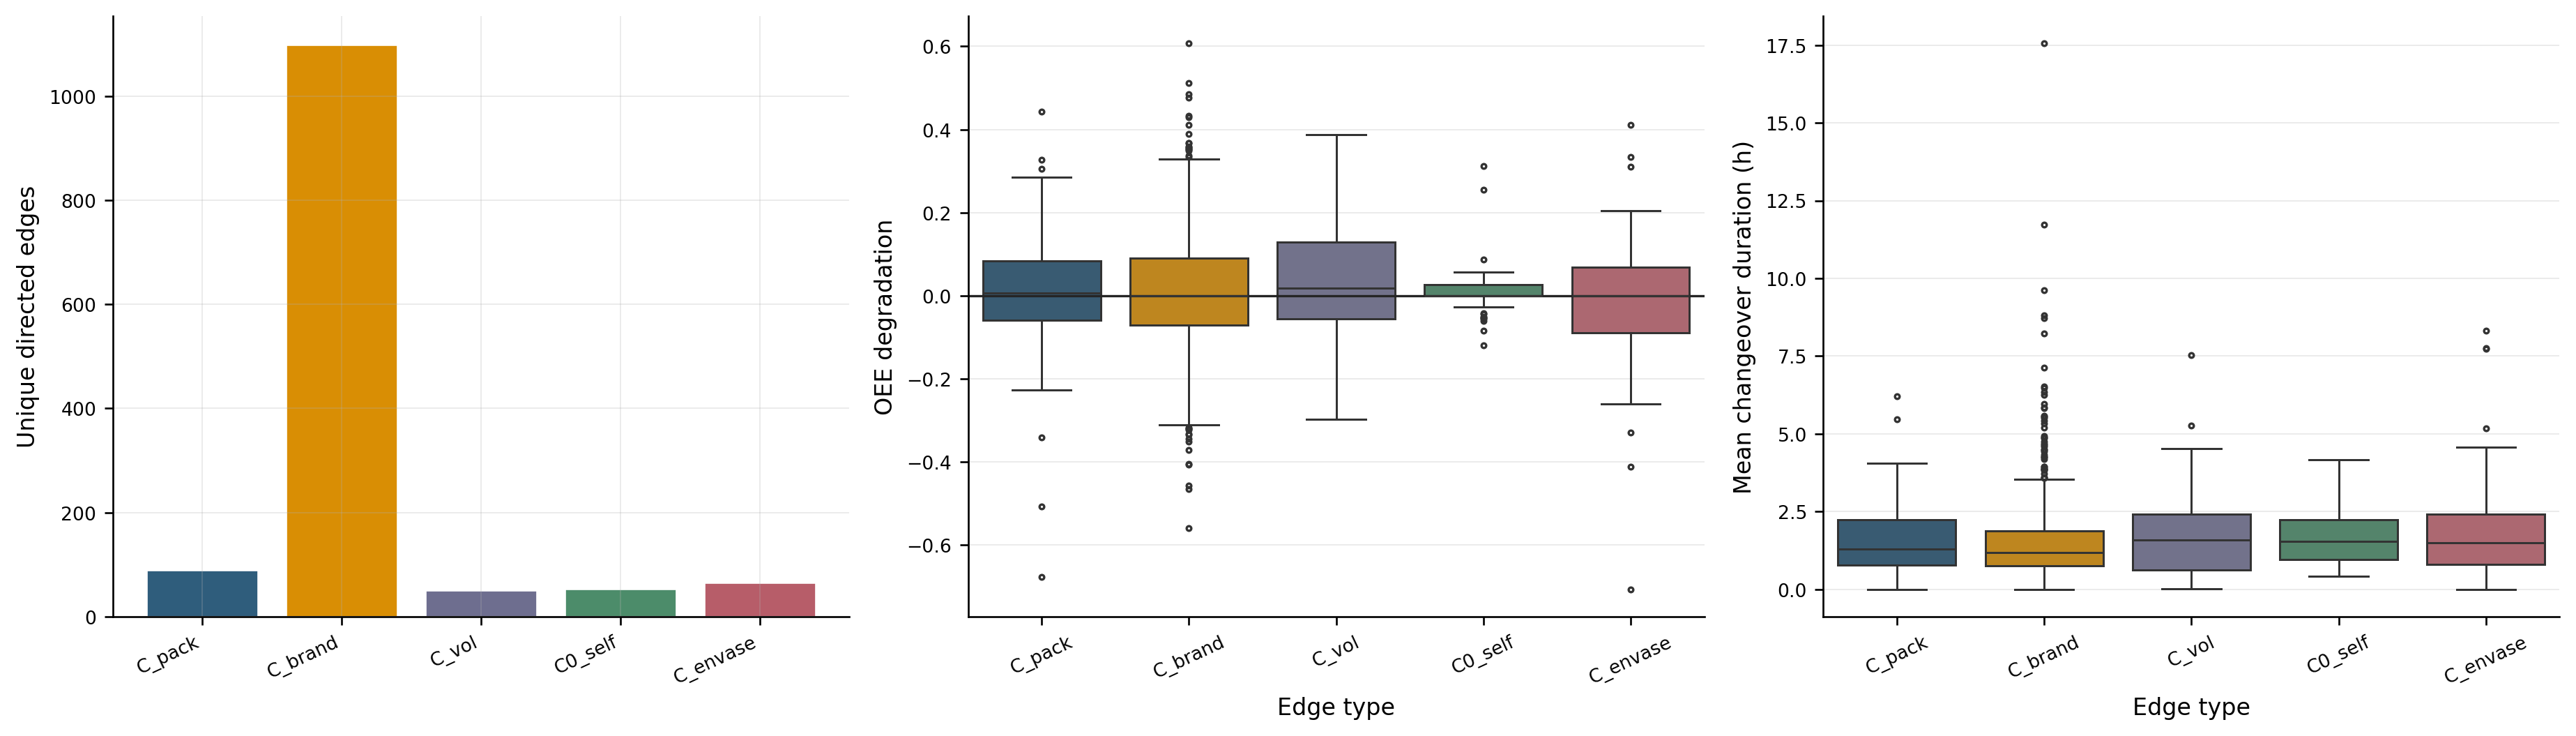
\includegraphics[width=\textwidth]{figures/nb02_fig01.png}
\caption{Directed changeover graph (per line).}
\end{subfigure}\hfill
\begin{subfigure}{0.49\textwidth}\centering
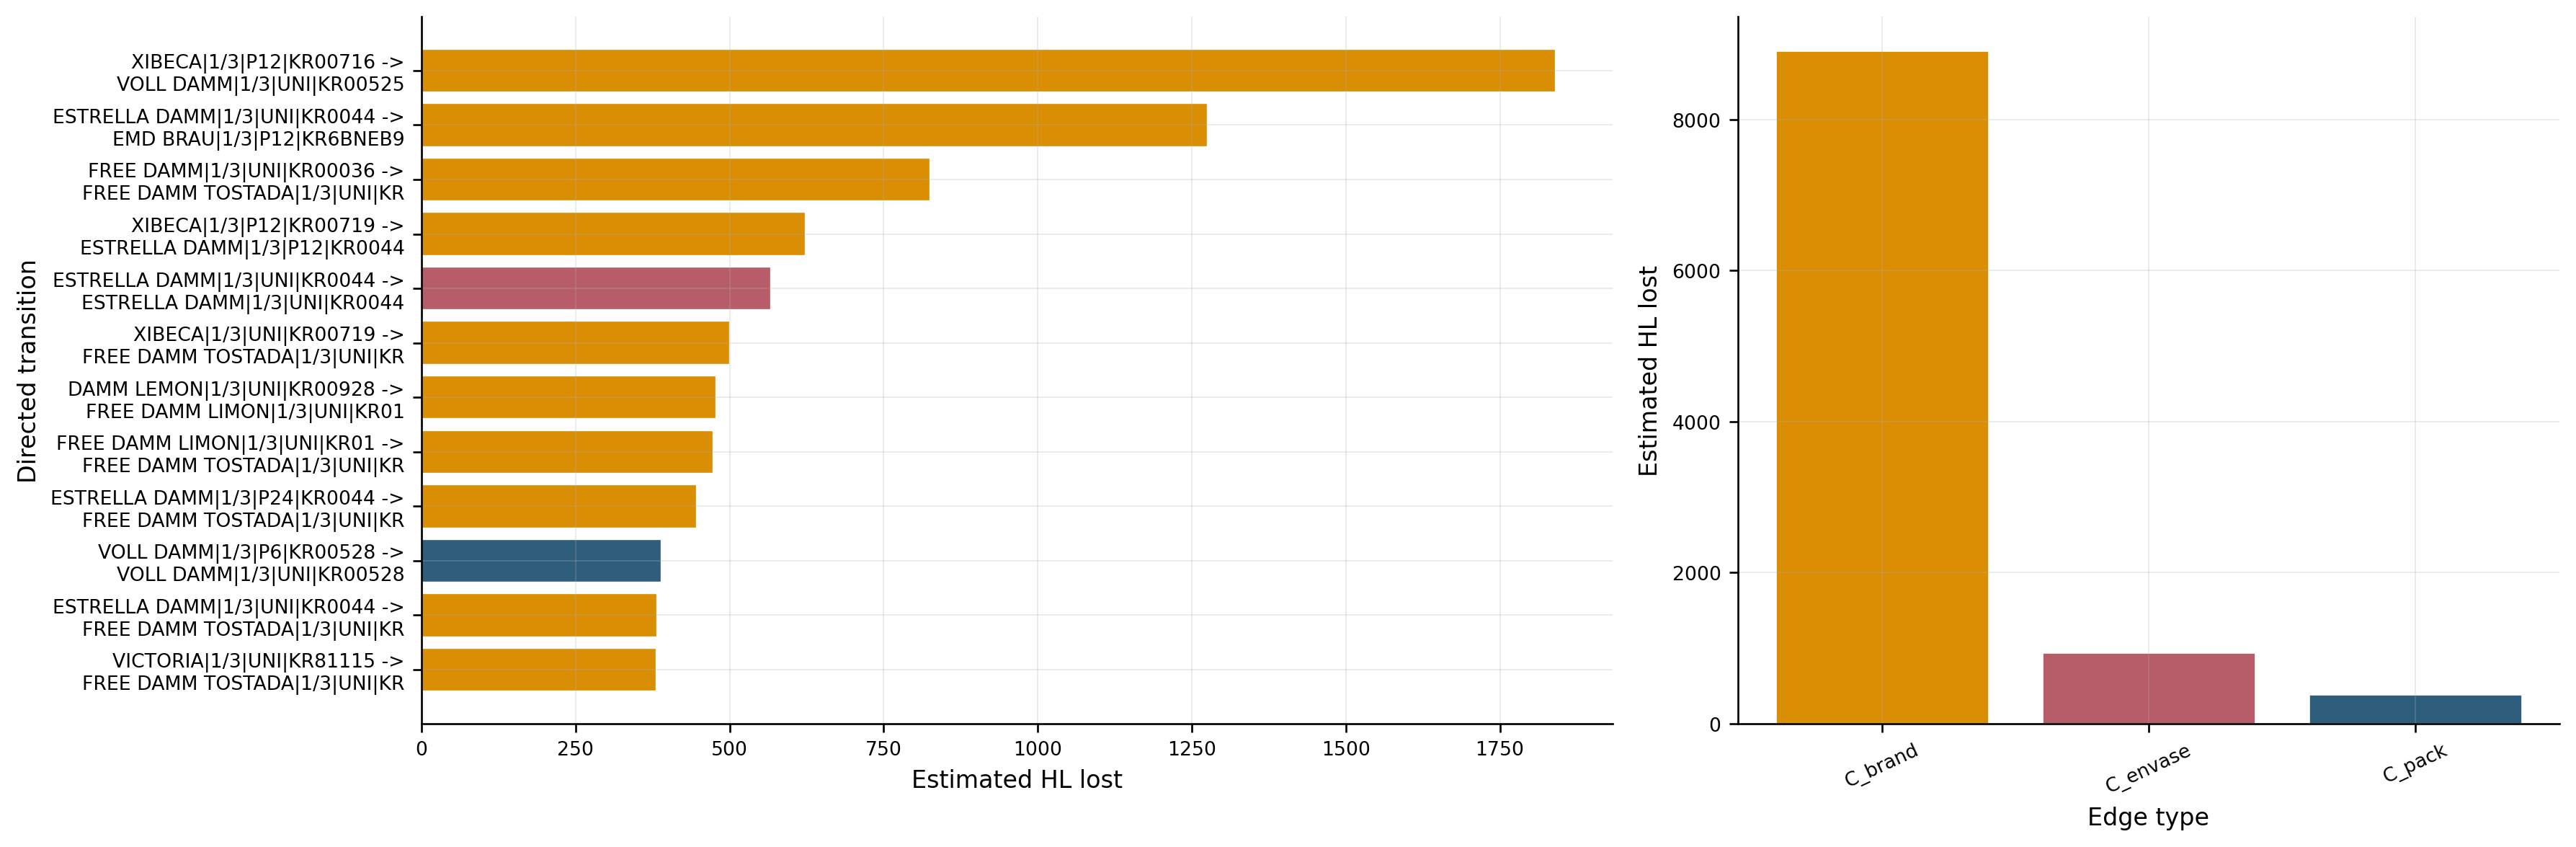
\includegraphics[width=\textwidth]{figures/nb02_fig02.png}
\caption{Black-spot ranking by estimated hL lost.}
\end{subfigure}
\caption{Post-mortem of the 2025 history: the directed transition graph and the
ranked black spots that drive avoidable loss.}
\label{fig:postmortem}
\end{figure}

\paragraph{Weekly schedule.}
For the target week ($28$ SKUs, $36{,}933$\,hL) all three engines converge to the
\emph{same} feasible plan: a total of $\mathbf{267.05}$\,h leaving
$\mathbf{72.95}$\,h of weekly slack (Table~\ref{tab:sched}). That the
heuristic GA and the exact CP-SAT model agree validates both the cost model and
the planner's manual baseline: the schedule is already near-optimal. The value of
the analysis is therefore not a dramatic re-shuffle but (i) the \emph{quantified
$73$\,h of head-room} for urgencies and demand swings, and (ii) the interpretable
rule of where to place expensive transitions (keep C\_envase off L14).

\begin{table}[H]\centering\small
\begin{tabular}{@{}lrrrrrr@{}}
\toprule
Line & SKUs & Prod (h) & Changeover (h) & Total (h) & Capacity (h) & Slack (h)\\
\midrule
L14 & 3  & 68.62 & 2.00  & 70.62  & 110 & 39.38 \\
L17 & 12 & 83.96 & 11.00 & 94.96  & 115 & 20.04 \\
L19 & 13 & 89.47 & 12.00 & 101.47 & 115 & 13.53 \\
\midrule
\textbf{Total} & 28 & 241.95 & 25.00 & \textbf{267.05} & 340 & \textbf{72.95}\\
\bottomrule
\end{tabular}
\caption{Optimised weekly schedule (identical across CP-SAT, graph and GA). All
lines feasible; $72.95$\,h of slack recovered against the contractual capacity.}
\label{tab:sched}
\end{table}

\paragraph{Plan versus reality.}
Reconciling the plan with the as-built log of 18--22 May 2026 gives an overall
attainment of $\mathbf{88.2\%}$ ($38{,}495$\,hL produced of $43{,}659$\,hL
planned; Table~\ref{tab:planreal}). The shortfall is uneven: L17 reached only
$74.4\%$ --- two SKUs (\texttt{SK13LN}, \texttt{VO13LTNN}) were never produced ---
while L19 overran to $105.9\%$, absorbing unplanned urgent SKUs. Re-optimising on
the \emph{realised} demand reproduces this stress exactly: L19 is the only
infeasible line ($117.67$\,h vs. $115$\,h, $-2.67$\,h), confirming that L19 acts
as the plant's buffer and is the binding constraint when urgencies arrive. When an
urgent order is added as a hard constraint (SKU must occupy an early position) the
optimiser either schedules it or, if it conflicts with format/eligibility/capacity,
\emph{reports infeasibility} rather than fabricating a solution --- the honest
behaviour an operations tool needs. Table~\ref{tab:realopt} shows the
re-optimisation on realised demand: L14 and L17 keep comfortable slack
($+46.5$ and $+19.4$\,h) while L19 alone breaches capacity, the quantitative
signature of the buffer role.

\begin{table}[H]\centering\small
\begin{tabular}{@{}lrrrrl@{}}
\toprule
Line & Prod (h) & Changeover (h) & Total (h) & Slack (h) & Feasible? \\
\midrule
L14 & 61.51 & 2.00  & 63.51  & $+46.49$ & yes \\
L17 & 85.62 & 10.00 & 95.62  & $+19.38$ & yes \\
L19 & 106.67& 11.00 & 117.67 & $-2.67$  & \textbf{no (over cap)} \\
\bottomrule
\end{tabular}
\caption{Re-optimisation on the \emph{realised} demand of 18--22 May 2026. Only
L19 exceeds its $115$\,h cap, confirming it as the binding constraint when
unplanned urgencies land.}
\label{tab:realopt}
\end{table}

\begin{table}[H]\centering\small
\begin{tabular}{@{}lrrrrr@{}}
\toprule
Line & hL plan & hL real & $\Delta$hL & Attainment & Real OEE\\
\midrule
L14 & 8{,}859.6  & 7{,}420.3  & $-1{,}439.2$ & 83.8\% & 0.59 \\
L17 & 18{,}297.4 & 13{,}605.9 & $-4{,}691.5$ & 74.4\% & 0.54 \\
L19 & 16{,}501.9 & 17{,}469.2 & $+967.3$     & 105.9\% & 0.64 \\
\midrule
\textbf{Total} & \textbf{43{,}658.9} & \textbf{38{,}495.4} & $-5{,}163.5$ & \textbf{88.2\%} & ---\\
\bottomrule
\end{tabular}
\caption{Plan vs. realised production (week 18--22 May 2026). L17 under-delivers,
L19 over-delivers as the urgency buffer.}
\label{tab:planreal}
\end{table}

% =====================================================================
\section{Findings, interpretation and conclusions}\label{sec:findings}
% =====================================================================
\paragraph{What the two methods jointly establish.}
Method~1 gives a \emph{trustworthy, self-updating cost per changeover}: a per-type
parametric law (not forced to Gamma), selected-family MCMC posteriors under
informative and weak priors (Table~\ref{tab:conv}), and a stationarity check that
licenses re-using the 2025 prior in 2026
(Table~\ref{tab:stat}). Method~2 turns that cost into \emph{actionable structure}:
a statistically certified ordering of changeover types and of lines
(Table~\ref{tab:summary}). The two agree on the central, counter-intuitive message
--- \textbf{a label-reference change (C\_envase) is the single most expensive
transition, costlier than a full brand change} --- and the directed-graph
post-mortem corroborates it through the centrality of label-heavy destination
nodes.

\paragraph{Operational consequences.}
\begin{enumerate}[leftmargin=1.6em,itemsep=1pt]
\item \emph{Sequencing rule:} group SKUs that share a label reference so C\_envase
transitions are rare; prefer C\_pack and C\_brand boundaries.
\item \emph{Line loading:} keep long, label-switching sequences off the slow L14,
and treat L19 as the urgency buffer it empirically is.
\item \emph{Targeted action:} the $21$ black spots ($\approx10{,}251$\,hL) are a
short, ranked worklist for SMED-style changeover reduction \cite{shingo1985smed}.
\item \emph{Planning value:} the optimiser confirms $\approx73$\,h of weekly slack
--- the quantitative room to absorb demand swings without overtime --- and the
plan-vs-real gap ($88\%$ attainment, L19 overshoot) pinpoints where that room
disappears.
\end{enumerate}

\paragraph{From evidence to action.}
Table~\ref{tab:actions} closes the loop by mapping each statistical result to the
concrete decision it licenses --- the deliverable a planner actually uses.

\begin{table}[H]\centering\small
\begin{tabular}{@{}lll@{}}
\toprule
Statistical evidence & Section & Operational action \\
\midrule
C\_envase is the costliest type ($p<0.01$) & \ref{sec:res-perm} & batch SKUs by label reference; minimise C\_envase \\
C\_brand $\approx$ C0\_self (plateau) & \ref{sec:res-perm} & treat brand changes and lot restarts as equal-cost \\
L14 slowest ($p<10^{-4}$) & \ref{sec:res-perm} & keep label-switching sequences off L14 \\
Process stationary (4/5 types) & \ref{sec:results} & reuse 2025 prior for 2026 planning \\
Informative vs. weak posterior comparison & \ref{sec:results} & historical prior stabilises sparse/long-tailed types \\
21 black spots, $\approx10{,}251$\,hL & \ref{sec:res-applied} & ranked SMED worklist \\
$72.95$\,h weekly slack & \ref{sec:res-applied} & head-room budget for urgencies \\
L19 binding under real demand & \ref{sec:res-applied} & route urgencies away from L19 when possible \\
\bottomrule
\end{tabular}
\caption{Traceability from statistical evidence to operational decisions.}
\label{tab:actions}
\end{table}

\paragraph{Quantified impact.}
The results convert into concrete numbers. The $21$ black spots represent an
estimated $10{,}251$\,hL of annual output lost to avoidable degradation; even a
partial SMED attack on the dozen worst transitions on L17 (the line carrying
$6{,}337$\,hL of that loss) targets the single largest recoverable pool. On the
forward-planning side, the $72.95$\,h of certified weekly slack is the buffer that
keeps the plant feasible under the demand swings the plan-vs-real analysis
exposed: when realised demand pushed L19 to $117.67$\,h the slack on L14 and L17
($46.5$ and $19.4$\,h) is exactly the capacity a re-balancing move would draw on.
The statistical layer thus pays for itself twice --- once by ranking where to cut
loss, once by quantifying the head-room that absorbs volatility.

\paragraph{Limitations.}
KS/CvM reject the parametric and stationarity nulls for C\_brand purely because
$n=508$ makes them over-powered; we therefore lean on AIC and effect size, not the
$p$-value alone. The hL impact of black spots is an estimate (degradation $\times$
volume), and the case$\rightarrow$hL conversion has known noise for three SKUs with
non-inferable format. Maintenance-contaminated OEE was median-imputed, which is
conservative but smooths genuine variance. C\_vol ($n=21$ overall, $15$ in $H_1$)
is too sparse for strong claims and is excluded from the ordered contrast. The
optimiser's eligibility is intentionally conservative (2025 precedent only), which
guarantees realism at the cost of never proposing a genuinely new SKU--line pairing.

\paragraph{Future work.}
Three extensions follow naturally. First, the per-edge empirical-Bayes priors could
be replaced by a fully \emph{hierarchical} model in which edge-, type- and
line-level effects are estimated jointly, sharpening the sparse arcs without the
hard $n\ge2$ cut-off. Second, the selected-family posterior cost could be pushed
into the CP-SAT objective as a risk-adjusted quantile (e.g.\ the posterior
$90\%$ duration) so the exact optimiser becomes robust, not just median-cost
optimal. Third, the
stationarity test could be run online as a change-point monitor, raising an alert
when a line's changeover distribution drifts --- closing the loop from descriptive
post-mortem to live process control.

\paragraph{Reproducibility.}
Every figure and number in this report is regenerated from the raw spreadsheets by
the executed notebook \texttt{07\_statistical\_analysis.ipynb} and the modules
\texttt{post\_mortem.py}, \texttt{ga\_optimizer.py} and
\texttt{scheduling\_cp\_sat.py}; the statistical routines are reproduced verbatim
in Appendix~\ref{sec:appendix}. Fixed random seeds make the $10{,}000$-permutation
nulls and the GA run deterministic, so the reported $p$-values and the $267.05$\,h
plan reproduce exactly.

\paragraph{Conclusion.}
A disciplined statistical treatment of an industrial log --- GoF-filtered
AIC-based family selection, selected-family Bayesian MCMC updating with an
explicit stationarity test, and distribution-free permutation tests for ordered alternatives ---
produced a validated, interpretable cost structure that both explains historical
losses and drives a feasible production schedule. Crucially, the statistical model
is not decorative: its posterior edge cost is the optimiser's cost oracle, and the
ordering it certifies is the rule the optimiser follows. The framework is
reproducible and self-improving: each new production week is one more observation
for the posterior of Eqs.~\eqref{eq:posterior_mcmc_inf}--\eqref{eq:posterior_mcmc_weak}, so the cost model --- and the
schedules it produces --- sharpen automatically as DAMM keeps operating.

% =====================================================================
\bibliographystyle{plain}
\bibliography{refs}

% =====================================================================
\appendix
\section{Appendix --- Reproducible analysis code}\label{sec:appendix}
% =====================================================================
The statistical analysis was implemented in \textbf{Python} (the language in which
the project was developed and executed). For full transparency,
Table~\ref{tab:software} maps every statistical procedure to its exact Python
package and function; the listings that follow contain the corresponding code. All
code, data and the executed notebook
(\texttt{notebooks/07\_statistical\_analysis.ipynb}) are reproducible end to end
with \texttt{numpy}, \texttt{pandas} \cite{mckinney2010pandas} and \texttt{scipy}
\cite{virtanen2020scipy} (SciPy 1.16, pandas 2.3).

\begin{table}[H]\centering\small\setlength{\tabcolsep}{4pt}
\begin{tabular}{@{}p{3.4cm}p{5.9cm}p{4.8cm}@{}}
\toprule
Procedure & Python function & Notes \\
\midrule
\multicolumn{3}{l}{\textit{Method 1 --- goodness of fit \& Bayesian inference}}\\
MLE fit of families & \texttt{scipy.stats.\{gamma,weibull\_min,} & location fixed: \texttt{.fit(s, floc=0)}\\
                    & \texttt{lognorm,invgauss\}.fit} & ($k=2$ free parameters)\\
AIC                 & \texttt{-2*dist.logpdf(s,*p).sum()+2k} & Eq.~\eqref{eq:aic}\\
Kolmogorov--Smirnov (1-sample) & \texttt{scipy.stats.kstest} & GoF vs.\ fitted CDF\\
Cram\'er--von Mises (1-sample)  & \texttt{scipy.stats.cramervonmises} & uniform-weight GoF\\
KS (2-sample, $H_1$ vs $H_2$)  & \texttt{scipy.stats.ks\_2samp} & stationarity\\
Anderson--Darling (k-sample)   & \texttt{scipy.stats.anderson\_ksamp} & tail-weighted\\
Cram\'er--von Mises (2-sample) & \texttt{scipy.stats.} & stationarity\\
                    & \texttt{cramervonmises\_2samp} & \\
Selected-family posterior      & custom \texttt{mh\_sampler} & Metropolis--Hastings on log-parameters\\
Posterior cost summary         & custom \texttt{duration\_mean} & median and 95\% credible interval\\
\midrule
\multicolumn{3}{l}{\textit{Method 2 --- permutation tests}}\\
Joint ranks            & \texttt{scipy.stats.rankdata} & mean within-group ranks\\
Label-permutation null & \texttt{numpy.random.Generator.} & $10{,}000$ resamples\\
                    & \texttt{permutation} & \\
Line post-hoc          & \texttt{scipy.stats.mannwhitneyu} & one-sided, Bonferroni\\
Pair enumeration       & \texttt{itertools.combinations} & $\binom{4}{2}$ ordered pairs\\
\bottomrule
\end{tabular}
\caption{Software-and-methods map: each statistical test and the Python function
that implements it. GoF and stationarity use \texttt{scipy.stats}; the
selected-family Bayesian posterior is sampled with a custom reproducible
Metropolis--Hastings routine.}
\label{tab:software}
\end{table}

\subsection{Data preparation, graph construction and goodness of fit}
\lstinputlisting[style=py]{appendix_code/01_data_and_gof.py}

\subsection{Bayesian selected-family MCMC updating}
\lstinputlisting[style=py]{appendix_code/02_bayesian_mcmc.py}

\subsection{Permutation tests for ordered alternatives}
\lstinputlisting[style=py]{appendix_code/03_permutation.py}

\end{document}
